% %%%%%%%%%%%%%%%%%%%%%%%%%%%%%%%%%%%%%%%%%%%%%%%%%%%%%%%%%%%%%%%%%%%%%%%%%%%%%%
% PREAMBLE

\documentclass[twoside, openany, 10pt]{report}


% ------------------------------------------------------------------------------
% Variables

% Title for the title page 
\newcommand{\thesisTitle}{Requirements Analysis and Specification Document}
% Title for the pages' heading 
\newcommand{\thesisTitleShort}{RASD}

\newcommand{\thesisSubtitle}{Best Bike Paths}

\newcommand{\thesisType}{Project report}  % Bachelor's Thesis, Master's Thesis, PhD Thesis...
\newcommand{\thesisDegree}{Master's Degree}  % Bachelor's Degree, Master's Degree, PhD...
\newcommand{\thesisArea}{Computer Science and Engineering}  % Area of knowledge

\newcommand{\thesisAuthor}{Daniele Toniolo - Stefano Ungaro - Matteo Zappa}

\newcommand{\thesisDate}{{\thesisMonth} {\thesisYear}}
\newcommand{\thesisAcademicCourse}{2025/2026}  % During which academic year(s) was the thesis developed

\newcommand{\thesisSchool}{Politecnico di Milano}
\newcommand{\thesisAddress}{Piazza Leonardo da Vinci, 32, 20133 Milano (MI), Italia}
\newcommand{\thesisDepartment}{Scuola di Ingegneria Industriale e dell'Informazione}

\newcommand{\thesisKeywords}{Keyword 1, Keyword 2, Keyword 3, Keyword 4, Keyword 4, Keyword 5, Keyword 6, Keyword 7, Keyword 8, Keyword 9, Keyword 10, Keyword N}  
% For the abstract and indexing


% ------------------------------------------------------------------------------
% Import document style
\usepackage{style/alcazar}

\begin{document}
% Titlepage, abstract and tables of contents
% Title page
\thispagestyle{empty}

\pagenumbering{Roman}
\setcounter{page}{1}


\newgeometry{
    left    = 3.0cm,
    right   = 3.0cm,
    top     = 3.5cm,
    bottom  = 3.5cm
}


\begin{center}
    
\includegraphics[width=\textwidth]{opening/logos/logo.pdf}
\end{center}

\vspace*{30mm}

\begin{center}
    \textbf{\large \textsc{{\thesisDegree} in}}\\
    \textbf{\large \textsc{\thesisArea}}
\end{center}

\vspace*{0mm}

\begin{center}
    \textbf{\large \thesisType}
\end{center}

\vspace*{20mm}

\begin{center}
    \setstretch{1.7}
    \textbf{{\LARGE {}``\thesisTitle''}}\\
\end{center}

\begin{center}
    \setstretch{1.7}
    \textbf{{\Large {}``\thesisSubtitle''}}\\
\end{center}

\vspace*{20mm}

\begin{center}
    {\large \textsc{Academic Year:} \thesisAcademicCourse}
\end{center}

\vspace*{20mm}

\begin{center}
    \begin{tabular}{rll}
        Authors: & \textbf{\large Daniele Toniolo} & \textbf{\large([redacted])} \\
                 & \textbf{\large Stefano Ungaro} & \textbf{\large([redacted])} \\
                 & \textbf{\large Matteo Zappa} & \textbf{\large([redacted])} \\
                 \\
        Professor: & \textbf{\large Matteo Camilli} & \\
    \end{tabular}
\end{center}

\newpage
\thispagestyle{empty}
\restoregeometry


% Table of contents
\newpage
\thispagestyle{empty}

%\clearpage
%\cleardoublepage
%\phantomsection

\pagestyle{plain}


\begingroup

    % Greatly compress space used by TOC, LOF and LOT
    \renewcommand{\baselinestretch}{1}  % less spacing
    \small  % smaller font size
    \setlength{\parskip}{0mm}  % Paragraph skip 0mm

    % List of Contents
    {
        \hypersetup{linkcolor=black}
        \addcontentsline{toc}{chapter}{Table of Contents}
        \tableofcontents
        \newpage
        \addcontentsline{toc}{chapter}{List of Figures}
        \listoffigures
        \newpage
        \addcontentsline{toc}{chapter}{List of Tables}
        \listoftables
    }
    

    
\endgroup

% Chapters
% Start standard numbering and page style

%\clearpage
%\cleardoublepage
%\phantomsection

\pagestyle{chapters}
\pagenumbering{arabic}
\setcounter{page}{1}

\chapter{Introduction}

\section{Purpose}
Cycling enthusiasts and daily commuters often face significant challenges in identifying safe and reliable routes for their journeys, as standard navigation tools frequently lack granular information regarding the physical condition of roads.

Best Bike Paths (BBP) is designed to fill this problem. The Platform aims to assist cyclists in their activities by creating a dynamic, crowdsourced inventory of bike Paths while enabling the community to effectively share data about Path statuses and obstacles. By addressing the mismatch between static map data and the actual road conditions, BBP enhances the routing process, creating an ecoSystem where User participation directly translates into safer and more informed cycling experiences.

\subsection{Goals}
\begin{glist}
    \item Cyclists should be assisted in their cycling activities through the analysis of their Trips.
    \item Cyclists should be able to record their Trips.
    \item Cyclists should be able to view their Trips' analysis based on performance (\eg, speed, time, total distance) and on Paths (\eg, status, presence of obstacles, weather).
    \item Cyclists should be able to provide information on Paths statuses manually.
    \item Cyclists should have their Trips' Paths automatically recorded while cycling.
    \item Cyclists should be able to access reliable and consolidated information about Paths (\eg, status, score) derived from the aggregation of community data.
    \item Cyclists should be able to obtain a list of possible Paths from a source point to a destination point, along with their scores and statuses.
    \item Cyclists should be able to suggest Paths to other Users.
\end{glist}

\section{Scope}

Best Bike Paths (BBP) is a collaborative Platform designed to enhance the cycling experience by facilitating the collection and retrieval of granular road information. It serves a dual purpose: enabling Registered Users to track their performance and actively contribute to the community, while allowing Guest Users to safely navigate and explore the existing map inventory.

At the core of the System lies the Data Aggregation logic. By collecting heterogeneous User reports on road Segments (\eg, \emph{Optimal}, \emph{Needs Maintenance}), the Platform resolves conflicting information based on data freshness and confirmation counts, ultimately assigning a single, reliable quality score to each route.

To minimize User distraction and ensure data accuracy, the System automates key activities such as obstacle detection via accelerometer and gyroscope analysis, weather data retrieval, and performance statistics calculation. Furthermore, it provides dedicated tools for the manual validation of anomalies and the management of personal Trip history, ensuring a comprehensive and reliable service.
\subsection{World Phenomena}
\begin{wplist}
    \item Users choose their preferred Path suggestion among a list of alternatives.
    \item Users start a cycling Trip.
    \item Users end a cycling Trip.
    \item During a ride, Users encounter obstacles along the way, such as potholes.
    \item The Users' mobile devices undergo physical vibrations and orientation changes while cycling.
    \item Paths conditions worsen during time.
    \item Municipalities or entities improve the physical state of Paths through maintenance or new constructions.
    \item Information regarding weather conditions is collected and made available by external meteorological services.
    \item Users decide to plan a Trip between two locations.
    \item Users decide to have their Trip recorded for analysis.
\end{wplist}

\subsection{Shared Phenomena}

\subsubsection*{World Controlled}
\begin{splist}
    \item Users enter credentials to sign up to BBP.
    \item Users enter credentials to log in to BBP.
    \item Users enter the application without providing credentials (Guest access).
    \item Users manually provide details about Paths.
    \item Users begin a cycling session on BBP.
    \item Users end a cycling session on BBP.
    \item Users confirm the presence of an automatically detected obstacle.
    \item Users deny the presence of an automatically detected obstacle.
    \item Users delete a Trip.
    \item Users make their Trips' Path information public.
    \item Users insert a source point for Path research.
    \item Users insert a destination point for Path research.
    \item The User's mobile device transmits GPS coordinates to the System.
    \item The User's mobile device transmits accelerometer and gyroscope data to the System.
    \item The External Meteorological Service transmits weather data to the System.
\end{splist}

\subsubsection*{Machine Controlled}
\begin{splist}[resume]
    \item The System displays automatically detected obstacles to the User for confirmation.
    \item The System provides the Users with possible Paths from a source to a destination, including their scores.
    \item The System displays performance statistics (\eg, speed, distance) to the User.
    \item The System requests weather updates for a specific location to the External Meteorological Service.
\end{splist}

\section{Definitions, Acronyms, Abbreviations}

\subsection{Definitions}
\begin{description}[noitemsep]
    \item [System, Platform] These terms are used interchangeably in this document to refer to the Best Bike Paths (BBP) software and infrastructure.
    
    \item [Trip] A continuous cycling activity recorded by a specific User, characterized by a temporal sequence of GPS coordinates and associated sensor data.

    \item [Segment] The atomic unit of a Path (\eg, a stretch of road between two intersections or a trail section). 
    
    \item [Path] A logical sequence of geographical Segments connecting a starting point to a destination, which can be traversed by a bicycle. It is the static representation of a route, distinct from the dynamic \emph{Trip} which is the act of traversing it.
    
    
    \item [Obstacle] A physical anomaly detected along a Path that represents a non-optimal condition for riding. Examples include, but are not limited to, potholes, steep slopes, speed bumps, and muddy terrain.
    
    \item [Status] A qualitative descriptor assigned to a Path or Segment (\eg, \emph{Optimal}, \emph{Sufficient}, \emph{Requires Maintenance}) derived from User reports and aggregated community data.
    
    \item [Score] A calculated numerical value representing the overall quality and efficiency of a Path. It is computed by the System based on the aggregated Status and other factors (\eg, obstacles) to rank search results.
    
    \item [Guest] An unregistered User who interacts with the Platform solely for information retrieval (searching Paths) without the ability to contribute data or record Trips.
\end{description}

\subsection{Acronyms}
\begin{table}[H]
    \sf
    \small
    \centering
    \renewcommand{\arraystretch}{1.5}
    \begin{tabularx}{\textwidth}{|l|X|}
        \hline
        \rowcolor{lightgray} \textbf{Acronym} & \textbf{Definition}\\
        \hline
        \textbf{BBP} & Best Bike Paths \\
        \textbf{RASD} & Requirements Analysis and Specification Document \\
        \textbf{API} & Application Programming Interface \\
        \textbf{GPS} & Global Positioning System \\
        \textbf{OTP} & One Time Password \\
        \textbf{HTTPS} & HyperText Transfer Protocol over Secure Socket Layer \\
        \textbf{JSON} & JavaScript Object Notation \\
        \textbf{TLS} & Transport Layer Security \\
        \hline
    \end{tabularx}
    \caption{Acronyms used in this document}
\end{table}

\subsection{Abbreviations}
\begin{table}[H]
    \sf
    \small
    \centering
    \renewcommand{\arraystretch}{1.5}
    \begin{tabularx}{\textwidth}{|l|X|}
        \hline
        \rowcolor{lightgray} \textbf{Abbreviation} & \textbf{Definition}\\
        \hline
        \textbf{G} & Goal \\
        \textbf{WP} & World Phenomenon \\
        \textbf{SP} & Shared Phenomenon \\
        \textbf{DA} & Domain Assumption \\
        \textbf{R} & Requirement \\
        \textbf{UC} & Use Case \\
        \hline
    \end{tabularx}
    \caption{Abbreviations used in this document}
\end{table}

\section{Revision History}
\begin{table}[H]
    \sf
    \small
    \centering
    \renewcommand{\arraystretch}{1.5}
    \begin{tabularx}{\textwidth}{|l|l|X|}
        \hline
        \rowcolor{lightgray} \textbf{Revised on} & \textbf{Version} & \textbf{Description}\\
        \hline
        23/12/2025 & 1.0 & Initial release of the document \\
        \hline
    \end{tabularx}
    \caption{Revision history of this document}
\end{table}

\section{Reference Documents}
The information contained in this document is based on the following sources:
\begin{enumerate}[noitemsep]
    \item Di Nitto, Rossi, Camilli, \emph{"A.Y. 2025-2026 Software Engineering 2 Requirement Engineering and Design Project"}, 2025.
    \item ISO/IEC/IEEE 29148:2018 - ISO/IEC/IEEE International Standard, \emph{"Systems and software engineering - Life cycle processes - Requirements engineering"}, 2018.
\end{enumerate}

\section{Document Structure}
\begin{description}
    \item [1. Introduction] a brief description of the project derived from the analysis of the provided specifications; it highlights the product's goals and scope.
    \item [2. Overall Description] a more detailed description of the product that includes real-world scenarios and analyses the System from a technical perspective.
    \item [3. Specific Requirements] a detailed list of all requirements necessary to satisfy the project goals, and their relationship with domain assumptions.
    \item [4. Formal analysis using Alloy] a formal description of a subset of real-world phenomena, analysed using Alloy to highlight inconsistencies between assumptions and the previously modelled phenomena.
    \item [5. Effort spent] the time spent by each group member contributing to the creation of this document.
    \item [6. References] references to documents or tools used in the preparation of this document.
\end{description}

\chapter{Overall Description}

\section{Product perspective}

\subsection{Scenarios}

\subsubsection*{Scenario 1: Automated Recording and Sensor-based Detection}
Daniele, an enthusiast cyclist, wants to track his daily commute to work. He opens the BBP app, logs in, and selects \emph{Start Cycling}. As he rides, the System automatically records his GPS Path. Suddenly, he hits a deep pothole; his smartphone vibrates violently. The System's algorithm analyses the accelerometer and gyroscope data and flags a potential obstacle at that location.

Upon reaching her destination, Daniele selects \emph{End Cycling}. The System presents a summary of the Trip, including performance statistics (speed, duration) and weather data (sunny, 22°C) retrieved from the external meteorological service. The System also asks him to validate the detected anomaly: \emph{We detected a strong vibration. Was this a pothole?}. Daniele confirms the detection. Finally, he decides to make this Path data public to warn other cyclists.

\subsubsection*{Scenario 2: Trip Planning with Data Merging and Freshness Analysis}
Stefano wants to plan a safe Sunday ride from his home to the city park. He navigates to the \emph{Discover} section and enters the source and destination points. The System calculates possible routes based on the available public data.

One direct route exists, but the System marks it with a low score and a \emph{Needs Maintenance} status. This happens because, although two Users rated it as \emph{Optimal} last month, three new Users reported \emph{Severe Potholes} yesterday. The System's merging algorithm prioritizes this fresher, confirming data. Consequently, BBP suggests an alternative, slightly longer route that has a high score and \emph{Optimal} status confirmed by recent Trips. Stefano chooses the safer alternative.

\subsubsection*{Scenario 3: Manual Path Creation and Management}
Matteo, an expert mountain biker, knows a shortcut through a forest trail that isn't mapped on standard road maps. He is currently at home and cannot ride it, so he logs into BBP and selects the \emph{Create a Path} section. 

Interacting with the map, he manually inputs the sequence of Segments connecting the entrance and exit of the trail. He assigns a specific status (\emph{Difficult}, \emph{Muddy}) to the route, which the System applies to all the involved Segments. Since he wants to immediately share this discovery with the community, he sets the visibility to \emph{Public} and confirms the creation. The System saves the Path and immediately updates the global map aggregation.

\subsubsection*{Scenario 4: Registration and Profile Setup}
Michele is a new User who wants to join the community. He downloads the app and selects \emph{Sign Up}. He provides his email, name, and password. After receiving an OTP code via email and verifying his identity, his account is active. He then accesses his profile to set his preferences. He is now ready to record Trips or browse the existing inventory of bike Paths.

\subsubsection*{Scenario 5: Guest Exploration (The Tourist)}
Tommaso is a tourist visiting the city for a weekend. He rents a bike and downloads BBP to find a safe route to the castle, but he does not want to create an account or share his personal details.

He selects \emph{Guest Login} (or \emph{Skip Registration}). The System allows him to access the \emph{Discover} section and search for Paths. He finds a highly-rated route and follows it using the map. However, when he tries to press \emph{Start Cycling} to record his performance, the System informs him that this feature requires a registered account. Tommaso declines the registration and continues to use the app solely for navigation and browsing public information.

\subsubsection*{Scenario 6: Smart Activity Detection and Trip Deletion}
Daniele starts a new recording for a training session. During the ride, he encounters a red traffic light and stops; the BBP System detects the zero speed and automatically pauses the recording to preserve the accuracy of the performance statistics. Later, he decides to get off the bike and walk it across a pedestrian area to grab a coffee. The System analyzes the accelerometer patterns and GPS speed, correctly identifying the activity as \emph{Walking} rather than \emph{Cycling}, and keeps the recording paused, ensuring the pedestrian Segment is not added to the bike Path inventory.

When Daniele resumes cycling, the System automatically wakes up and continues the tracking. At the end of the day, reviewing his \emph{My Trips} section, Daniele realizes this fragmented session is not useful for his long-term statistics. Since the System design ensures data integrity by disallowing manual modification of the recorded GPS track structure (to prevent data falsification), Daniele decides to discard the session entirely. He selects the Trip, taps \emph{Delete}, and confirms the action, permanently removing the data from the System.

\subsection{Domain Class Diagram}
The Domain Class Diagram (Figure \ref{fig:domain_class_diagram}) illustrates the conceptual model of the BBP System, defining the entities, their attributes, and the relationships that govern the System's logic. The model is designed to support the core requirements of crowdsourced data collection, Path reliability scoring, and User privacy.

\label{section:domain_class_diagram}
\begin{figure}[H]
    \centering
    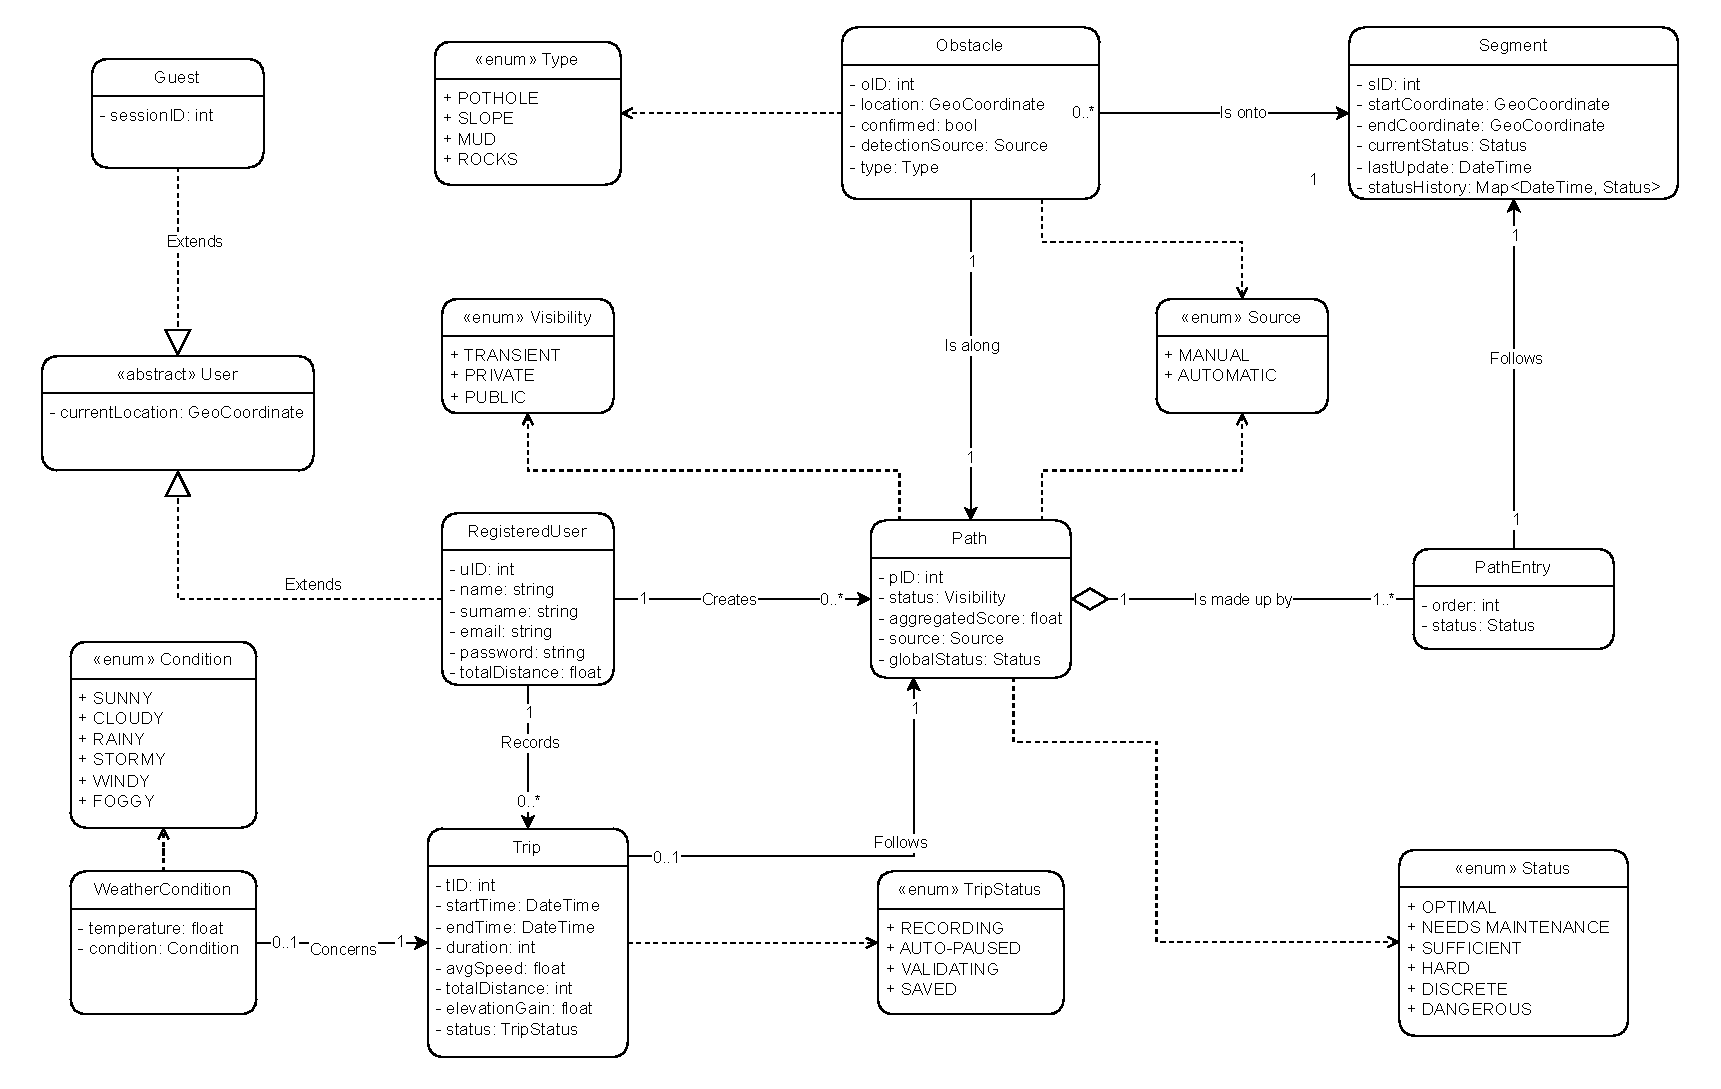
\includegraphics[width=0.99\textwidth]{pdf/domain_class_diagram.pdf}
    \caption{Domain Class Diagram for BBP}
    \label{fig:domain_class_diagram}
\end{figure}

The structure is centered around a clear separation between the \emph{Dynamic Activity} (the act of cycling) and the \emph{Static Geography} (the physical road network). This separation is crucial for the implementation of the Data Aggregation algorithm.

\subsubsection*{User Hierarchy}
The System defines a generalization hierarchy to manage different levels of access:
\begin{itemize}
    \item \textbf{User (Abstract)}: Represents the generalized concept of an actor interacting with the System via a mobile device. It holds the \texttt{currentLocation} (GeoCoordinate), which is the only attribute shared by all actors to enable map visualization and real-time tracking.
    \item \textbf{RegisteredUser}: Extends the generic User with persistent identity attributes (\texttt{email}, \texttt{password}), \texttt{name}, \texttt{surname}, and metrics such as \texttt{totalDistance}. This entity is the \emph{owner} of data: only a RegisteredUser can record \textbf{Trips} and create \textbf{Paths}.
    \item \textbf{Guest}: Represents an anonymous User. This entity has no persistent ID or profile data, consistent with the privacy-by-design approach, but inherits the capability to search and view the map. A \texttt{sessionID} is needed for session persistence.
\end{itemize}

\subsubsection*{Core Entities: Trip, Path, and Segment}
To satisfy the requirement of merging conflicting data from multiple Users while preserving the integrity of individual reports, the model adopts a normalized structure mediated by the \textbf{PathEntry} class:

\begin{itemize}
    \item \textbf{Trip}: 
    Represents the temporal event of a User cycling. It contains raw sensor data and performance metrics specific to that single session, such as \texttt{avgSpeed}, \texttt{totalDistance}, and \texttt{elevationGain}. 
    Crucially, it includes a \texttt{status} attribute (of type \texttt{TripStatus}) to track the recording lifecycle (\eg, Recording, Auto-Paused, Saved). A Trip is transient in nature; it documents \emph{what happened} at a specific time.
    
    \item \textbf{Path}: 
    Represents the immutable geographical definition of a route. It acts as a container for metadata such as \texttt{aggregatedScore} and \texttt{globalStatus}. 
    It holds a \texttt{status} attribute (of type \texttt{Visibility}) which manages the lifecycle and visibility of the route (\eg, Transient, Private, Public).
    The relationship between Trip and Path is defined as follows:
    \begin{itemize}
        \item A Trip \emph{follows} exactly one Path geometry (\texttt{1}).
        \item A Path is usually generated by a Trip, but can also be created manually without any recording. Hence, the multiplicity is \texttt{0..1} on the Trip side.
    \end{itemize}

    \item \textbf{PathEntry}: 
    This entity acts as the structural link between a user-defined Path and the physical road network. A Path is composed of a sequence of \texttt{PathEntries} (ordered by the \texttt{order} attribute).
    Crucially, \texttt{PathEntry} holds the \texttt{status} assigned by the user during that specific trip. This ensures that the user's subjective rating is encapsulated within their private Path data and is only propagated to the global map when the Path becomes Public.

    \item \textbf{Segment}: 
    This is the core entity for the \textbf{Data Aggregation} logic. A \texttt{Segment} represents a physical, atomic stretch of road (\eg, a specific street block or trail section) that exists independently of any User. 
    \begin{itemize}
        \item \textbf{Aggregation Logic}: The Segment holds the \texttt{currentStatus} (\eg, \emph{Muddy}) and the \texttt{lastUpdate} timestamp, representing the "global truth" visible to all users.
        \item \textbf{Status Propagation}: When a Path is published, the aggregation algorithm iterates through the list of \texttt{PathEntries}, taking the user-specific ratings and merging them into the \texttt{currentStatus} of the corresponding Segments. The Segment also maintains a \texttt{statusHistory} map to allow for data rollback and validation.
    \end{itemize}
\end{itemize}

\subsubsection*{Context and Anomalies}
The model includes entities to capture the environmental context of the ride:

\begin{itemize}
    \item \textbf{Obstacle}: Represents a hazard (\eg, \emph{Pothole}, \emph{Slope}) detected along a route. Obstacles lie on specific Segments and are connected to a specific Path.
    Crucially, the Obstacle includes a \texttt{detectionSource} attribute (defined in the \texttt{Source} enumeration) to distinguish between anomalies automatically detected by the sensors (accelerometer/gyroscope) and those manually inserted by the User during validation.
    
    \item \textbf{WeatherCondition}: Associated with every Trip, when available, it freezes the meteorological conditions (Temperature, Condition) at the time of the recording. This allows the System to filter statistics (\eg, \emph{Performance on rainy days}).
\end{itemize}

\subsubsection*{Enumerations}
To ensure data consistency, the model relies on strict enumerations for categorical data:
\begin{itemize}
    \item \textbf{Status}: Defines the quality of a Segment (Optimal, Sufficient, Hard, Dangerous).
    \item \textbf{Type}: Classifies the hazards (Pothole, Mud, Rocks).
    \item \textbf{Condition}: Standardizes weather reports (Sunny, Rainy, Foggy).
    \item \textbf{Source}: Distinguishes between Manual and Automatic obstacle detection.
    \item \textbf{TripStatus} and \textbf{Visibility}: Define the lifecycle states for the respective entities.
\end{itemize}
These enumerations can be extended with additional entries for a more detailed representation of different aspects of the object they refer to.
\subsection{State Diagrams}
To clarify the dynamic behaviour of the System's core entities, the following state diagrams illustrate the lifecycle of a \textbf{Trip} (focusing on the recording logic) and a \textbf{Path} (focusing on data persistence and visibility).


\subsubsection*{Trip Lifecycle}
Figure \ref{fig:Trip_state_diagram} models the User's recording session. It highlights the \emph{Smart Pausing} mechanism defined in requirement [R9], ensuring that stops or non-cycling activities do not pollute the performance statistics.

\begin{itemize}
    \item \textbf{Recording}: The active state where the System logs GPS coordinates and sensor data.
    \item \textbf{Auto-Paused}: Entered automatically when the System detects the speed has dropped below a threshold (for example, if the User is walking). In this state, data logging is suspended. The System automatically reverts to \emph{Recording} once cycling resumes.
    \item \textbf{Validating}: A transitional state entered upon pressing the \emph{Stop} button. Here, the data is frozen while the User confirms details about the Path and assigns a status (as per UC5). From here, the User can either confirm the session or discard it entirely.
    \item \textbf{Saved}: The final stable state where the Trip is persisted in the User's history (\emph{My Trips} section). It remains here until the User explicitly decides to delete it.
\end{itemize}

\subsubsection*{Path Lifecycle}
Figure \ref{fig:Path_state_diagram} illustrates the lifecycle of the geographical route definition, managing its visibility to the community. This logic is central to the \emph{Data Merging} requirements.

\begin{itemize}
    \item \textbf{Transient}: The Path is being defined (either by a recording session or manual drawing via UC7) but is not yet persisted in the database. If the creation is cancelled, the object is destroyed.
    \item \textbf{Private}: The Path is visible only to its creator and does not contribute to the global map statistics.
    \item \textbf{Public}: The User has explicitly shared the Path. In this state, the Path's Segment statuses are merged into the global heatmap using the aggregation algorithm. A Path can be toggled between \emph{Private} and \emph{Public} at any time, triggering a recalculation of the community data.
\end{itemize}


\begin{figure}[H]
    \begin{subfigure}{\textwidth}
        \centering
        \includegraphics[width=\textwidth]{pdf/Trip_state_diagram.pdf}
        \caption{State Diagram of a Trip}
        \label{fig:Trip_state_diagram}    
    \end{subfigure}
    \begin{subfigure}{\textwidth}
        \centering
        \includegraphics[width=\textwidth]{pdf/Path_state_diagram.pdf}
        \caption{State Diagram of a Path}
        \label{fig:Path_state_diagram}
    \end{subfigure}
    \caption{State Diagrams for Core Entities}
\end{figure}
\newpage
\section{Product functions}
The BBP Platform is designed to help cyclists manage their Trips and Paths flawlessly, with key features that help make the User experience friendly and optimal for monitoring and planning.

\begin{itemize}
    \item \textbf{User Access and Registration}: Users can sign up to the Platform to enable tracking features and contribute to the community data. The System also supports a \emph{Guest Mode}, allowing unregistered Users to browse the inventory and search for Paths without recording their activities.
    
    \item \textbf{Trip Tracking and Statistics}: The Platform provides a tracking functionality that Users can activate when starting a new Trip. While cycling, the application uses the built-in phone sensor System (GPS, accelerometer, gyroscope) to record the session and analyse performance (\eg, speed, duration). If available, the System enriches the Trip data with meteorological information retrieved from external services.
    
    \item \textbf{Automated Data Acquisition}: During a Trip, the System automatically detects the Path structure and identifies potential anomalies (\eg, potholes) by analysing sensor data. It features activity recognition to distinguish whether the User is cycling based on speed and movement patterns.
    
    \item \textbf{Data Validation}: To mitigate false positives in automated detection, the System provides an interface for Users to review, confirm, or correct the automatically detected obstacles and Path Segments before saving or publishing the Trip.
    
    \item \textbf{Manual Path Management}: The System allows Users to define Paths manually without cycling, by selecting Segments on a map and assigning a status (\eg, \emph{Optimal}, \emph{Needs Maintenance}) which applies to the selected road sections. Users can manage the visibility of their Paths, choosing to keep them private or share them with the community.
    
    \item \textbf{Data Aggregation and Reliability Analysis}: The System processes public information incoming from different Users to create a consolidated view of the bike Paths network. It merges conflicting reports by considering data freshness and the number of confirming sources to assign a reliability score and a unified status to each Path.
    
    \item \textbf{Smart Path Search}: Users can search for Paths between two locations. The System visualizes the results on a map, filtering and ranking the alternatives based on the calculated score, Path status, and overall efficiency.
\end{itemize}

\subsection{Requirements}

\subsubsection*{Account and Session}
\begin{rlist}
    % --- ACCOUNT & SESSION ---
    \item Upon request, the System shall allow a User to sign up to the Platform, as long as they provide all the required information and a profile is not already associated with it.
    \item Upon request, the System shall allow a User to log in to the Platform, as long as the correct credentials are provided.
    \item Upon request, the System shall allow a User to access the Platform as a guest.
    \item Upon request, the System shall allow a registered User to start a training session.
    \item Upon request, the System shall allow a registered User to end a training session, as long as they had already started it before.
\end{rlist}

\subsubsection*{Recording and Sensors}
\begin{rlist}[resume]
    % --- RECORDING & SENSORS ---
    \item Whenever a Trip is being recorded, the System shall keep track of the Path followed by the User acquiring GPS coordinates.
    \item Whenever a Trip is being recorded, the System shall analyze data from the device's accelerometer and gyroscope to automatically detect potential obstacles (\eg, potholes).
    \item Whenever the System detects a potential obstacle during a recording, it shall temporarily store its location and type for validation at the end of the session.
    \item Whenever a Trip is being recorded, the System shall automatically pause the data acquisition if the detected speed or movement pattern suggests the User is not cycling (\eg, walking or stationary).
\end{rlist}

\subsubsection*{Validation and Immutability}
\begin{rlist}[resume]
    % --- VALIDATION & IMMUTABILITY ---
    \item Upon concluding a recorded Trip (and before final storage), the System shall require the User to validate (confirm or delete) the automatically detected obstacles and assign a general status to the traversed Segments.
    \item Upon concluding a recorded Trip (and before final storage), the System shall allow the User to manually insert and classify obstacles that were not automatically detected by the sensors.
    \item The System shall prevent any modification to the Path's structural data (GPS track) and descriptive details (status, obstacles) once the Path has been saved to the System.
\end{rlist}

\subsubsection*{Manual Management}
\begin{rlist}[resume]
    % --- MANUAL MANAGEMENT ---
    \item Upon request, the System shall allow a registered User to insert a Path manually, as long as a list of streets and statuses is provided.
    \item Upon request, the System shall allow a registered User to delete their recorded Trips.
    \item Upon request, the System shall allow a registered User to delete their Paths, whether inserted manually or automatically.
\end{rlist}

\subsubsection*{Visibility}
\begin{rlist}[resume]
    % --- VISIBILITY ---
    \item Upon request, the System shall allow a registered User to make their Path available to the community (public), as long as said Path is currently private.
    \item Upon request, the System shall allow a registered User to make their Path private, as long as said Path has already been shared with the community.
    \item Upon request, the System shall allow a registered User to view all their Trips and Paths, whether they are private or public.
\end{rlist}

\subsubsection*{Data Merging and Algorithms}
\begin{rlist}[resume]
    % --- MERGING & ALGORITHMS ---
    \item Whenever a Path is made public, the System shall recalculate the status of the involved street Segments by aggregating the User's data with existing community data.
    \item When aggregating conflicting data about a Path Segment, the System shall prioritize information based on its freshness (recency of submission).
    \item When aggregating conflicting data about a Path Segment, the System shall resolve inconsistencies by considering the number of confirming reports from different Users.
    \item Whenever a public Path is made private or deleted, the System shall remove the specific User's contribution from the aggregated community data, triggering a recalculation of the Segment's status.
\end{rlist}

\subsubsection*{Statistics and Information}
\begin{rlist}[resume]
    % --- STATS & INFO ---
    \item Whenever a Trip is recorded, the System shall elaborate statistics on performance, such as estimated speed, total length, and time.
    \item Whenever a Trip is concluded and external weather services are available, the System shall retrieve and store the weather conditions associated with the Trip's location and time.
\end{rlist}

\subsubsection*{Search}
\begin{rlist}[resume]
    % --- SEARCH ---
    \item Upon request, the System shall provide a list of Paths connecting two locations to any User (registered or guest), visualizing them on a map ordered by their calculated score.
    \item Whenever providing search results, the System shall calculate a Path's score based on its aggregated status (\eg, optimal vs. bad) and its effectiveness in reaching the destination.
\end{rlist}

\section{User characteristics}
The BBP Platform is designed for two distinct categories of Users, differentiated by their level of interaction with the System's database:

\begin{table}[H]
    \sf
    \small
    \centering
    \renewcommand{\arraystretch}{1.5}
    \begin{tabularx}{\textwidth}{|l|X|}
        \hline
        \rowcolor{lightgray} \textbf{User} & \textbf{Characteristics} \\
        \hline
        \textbf{Registered Cyclists} &
        \textbf{Description}: Individuals who actively use the Platform not only to find routes but also to record Trips, monitor performance, and contribute data to the community.
        They span from \emph{proficient Users}, familiar with fitness apps and navigation technology, to \emph{novice Users} who may be less experienced with such interfaces.

        \textbf{Interaction Frequency}: Expert cyclists typically access the Platform multiple times per week for training. Recreational Users show seasonal variability (higher activity in spring/autumn and weekends).
        
        \textbf{Key Role}: They are the primary source of information for the System (crowdsourcing). Therefore, their ability to easily confirm or correct automated data is crucial for the System's reliability. \\
        \hline
        \textbf{Unregistered Users (Guests)} &
        \textbf{Description}: Individuals who wish to access the public inventory of bike Paths for exploration without account creation or performance tracking.

        \textbf{Interaction Frequency}: Highly unpredictable. This category includes tourists using the app for a single weekend or casual Users evaluating the service before registering.

        \textbf{Key Role}: They act solely as information consumers and cannot contribute new data or modify existing Paths. \\
        \hline
    \end{tabularx}
    \caption{User characteristics}
\end{table}

Given that the User base ranges from highly technical Users to complete beginners, and considering that data quality relies on User validation, the Platform must ensure a high usability standard. The interface must be straightforward enough for a casual User to navigate without training, yet comprehensive enough to provide detailed analytics for the expert cyclist.

\section{Assumptions, dependencies and constraints}
\subsection{Regulatory policies}
Since the BBP Platform collects and processes sensitive User data, specifically real-time geolocation (GPS) and movement patterns (via accelerometer and gyroscope), compliance with the \emph{General Data Protection Regulation (GDPR)} is mandatory.
Specific policies include:

\begin{itemize}
    \item \textbf{Data Anonymization}: Before being merged into the public knowledge base or used for statistical analysis, raw Trip data must be anonymized to prevent the identification of specific individuals or their private locations (\eg, home addresses).
    \item \textbf{Purpose Limitation}: Data is collected strictly for the purpose of service provision (Trip tracking, Path analysis) and must not be used for third-party commercial profiling or sold to advertisers.
    \item \textbf{Explicit Consent}: The System must obtain explicit User consent before accessing device sensors and location services.
\end{itemize}

\subsection{Domain Assumptions}
\label{domain_assumptions}
\begin{dalist}
    \item Users' GPS location is accurate.
    \item Users interact with the BBP application through a device with a functioning GPS connection. 
    \item Cyclists that decide to sign up have access to the mailbox of the provided email address.
    \item Users do not provide harmful information on Paths, such as suggesting cycling in dangerous areas or malicious routes.
    \item The majority of Users participate in the community with the intent of providing accurate information. Consequently, statistical aggregation of conflicting reports converges towards the actual state of the Paths.    
    \item Cyclists follow local traffic laws (\eg no access to highways, motorways, or forbidden/private streets).    
    \item Cyclists travel along physically defined tracks (roads, bike lanes, or beaten trails) and do not traverse open terrain where no Path exists (\eg, cutting diagonally across a field).
    \item The external map provider's database used by the System includes all physical Paths suitable for cycling, including off-road trails that might be missing from standard street navigation maps.
    \item During a Trip, cyclists rely only on their bicycle and do not switch to other means of transport (\eg cars, trains, buses) without stopping the recording.
    \item An Internet connection is available for data synchronization (Log In, Upload, Search), although it may be intermittent or absent during the cycling activity itself.
\end{dalist}

\chapter{Specific Requirements}

\section{External Interface Requirements}
\subsection{User Interfaces}

\begin{figure}[H]
    \centering
    \includegraphics[width=0.9\textwidth]{pdf/User_interfaces.pdf}
    \caption{User Interfaces Map}
    \label{fig:User_interfaces}
\end{figure}
\newpage
\noindent
The Best Bike Paths (BBP) User interface shall be designed to be intuitive and strictly adherent to a \emph{map-centric} approach, considering that the application will be used primarily on mobile devices in outdoor settings. The interactions shall be optimized for single-handed usage and high legibility while moving.


In compliance with \hyperref[standards-compliance]{accessibility requirements} and store guidelines, the interface shall use high-contrast colour schemes, scalable fonts, and enlarged touch targets to facilitate interaction during physical activity.

\noindent
The main System screens are described below:

\begin{itemize}
    \item \textbf{Landing Screen (Authentication)}: 
    Upon launching the app, the User is presented with a mandatory \emph{Safety Disclaimer} regarding road risks. Once acknowledged, the screen offers clear entry points:
        \begin{itemize}
            \item \emph{Log In / Sign Up}: Standard input fields for registered Users to access their profile.
            \item \emph{Continue as Guest}: A prominent, high-visibility button allowing immediate access to map exploration without account creation.
        \end{itemize}

    \item \textbf{Home Dashboard}: 
    The central hub of the application, existing in two distinct versions: \emph{Guest Mode} (with restricted features) and \emph{Registered Mode} (providing full access).
        \begin{itemize}
            \item \emph{Interactive Map}: The core interface element occupying the majority of the screen, displaying the User's real-time position and nearby cycling Paths colour-coded by their aggregated status (\eg, Green for Optimal, Red for Damaged).
            \item \emph{Search Bar}: Floating at the top, allowing quick entry of source and destination points.
            \item \emph{Start Recording}: A large Floating Action Button to begin a Trip, available exclusively in Registered Mode.
            \item \emph{Bottom Navigation Bar}: Provides quick access to \emph{Explore}, \emph{Profile} and, for registered Users only, \emph{My Activity} (with subsections for Trips/Paths).
        \end{itemize}

    \item \textbf{Profile Section}: 
    Manages global application preferences and User session state. The interface adapts its content based on whether the User is Registered or navigating as a Guest.
    \begin{itemize}
        \item \emph{App Settings}: Manages app-specific technical configurations and privacy controls. While sensor usage consent is available to all, specific identity management features (\eg, GDPR data export, Account Deletion) are hidden for Guest Users.
        \item \emph{Authentication Controls}: A dynamic area that manages the current session status.
        \begin{itemize}
            \item For \textbf{Registered Users}, it displays a \emph{Logout} button to terminate the session.
            \item For \textbf{Guest Users}, it displays \emph{Log In} and \emph{Sign Up} buttons (or a banner) to encourage account creation and unlock full features.
        \end{itemize}
    \end{itemize}
    
    \item \textbf{Explore}: Serving as the application's main page for navigation, this section is centered around the \emph{Interactive Map}, which allows Users to browse the cycling network directly. It also provides access to the search functionality, detailed as follows:
    \begin{itemize}
        \item \textbf{Search Paths \& Results}: Upon entering a source and destination, the interface presents \emph{Path Alternatives} via a list or map overlay showing possible routes. Each option highlights the \emph{Score} (calculated by the merging algorithm) and the aggregated \emph{Status} , alongside \emph{Warnings} represented by icons indicating specific issues reported by the community (\eg, \emph{Muddy section}).
    \end{itemize}

    \item \textbf{My Activity}:
    This section is divided into two primary subsections:
    \begin{itemize}
        \item \textbf{My Trips Section}: Contains the chronological \emph{History List} of activities and the \emph{Trip Detail} view featuring graphs and maps, from which the \emph{Delete Trip} action can be performed. 
        \item \textbf{My Paths Section}: This section manages the repository of saved Paths, featuring a \emph{Path Library} that distinguishes between private and public entries. Users can access individual \emph{Path Details} to view metadata or execute the \emph{Delete Path} command to remove orphan Paths. 
        \begin{itemize} 
            \item \emph{Manual Path Creation}: Accessible here, it allows Users to define a Path without cycling via the \emph{Define Track} map editor and the \emph{Add Details} form for status and visibility. 
        \end{itemize}
    \end{itemize}

    \item \textbf{Recording Flow}:The tracking process is managed through two primary interfaces designed to minimize distraction and ensure data quality:
    \begin{itemize}
        \item \textbf{Active Recording Interface}: It is optimized for use while moving, displaying real-time metrics (speed, distance) and providing visual feedback for \emph{Auto-Pause} events. To prevent accidental interruptions during the ride, the \emph{Stop/Finish} function utilizes a deliberate ``slide-to-confirm'' interaction to terminate the session.
        \item Upon completion, the System presents the \textbf{Post-Ride Validation} screen, a critical summary for data aggregation displayed immediately after finishing a recording. In addition to presenting a final snapshot of performance statistics (duration, average speed) and the weather conditions automatically retrieved for the Trip's location , this interface allows the User to toggle the Path visibility between \emph{Private} and \emph{Public}  before finalizing the following data: 
        \begin{itemize} 
            \item \emph{Obstacle Validation}: A list allowing the User to confirm or reject anomalies automatically detected by the sensors. 
            \item \emph{Manual Obstacle Entry}: A specialized interaction allowing the User to manually drop a marker on the map to categorize obstacles that the automated sensors failed to detect during the ride.
            \item \emph{Path Rating}: A tool to assign a general status to the traversed Path (\eg, \emph{Optimal}). While this applies to all Segments by default, the User can override the status for specific map sections (\eg, marking a single stretch as \emph{Muddy}).
            \item \emph{Save/Delete Trip}: The final step to confirm saving the Trip to the database or permanently deleting the recording.
        \end{itemize}
    \end{itemize}
\end{itemize}

\subsection{Hardware Interfaces}
The BBP mobile application shall interact directly with specific hardware components embedded in the User's mobile device to fulfil its core functional requirements (tracking and sensing). The interactions are managed through the abstraction layers provided by the mobile operating System:

\begin{itemize}
    \item \textbf{Global Navigation Satellite System (GNSS) Receiver}:
    The application shall interface with the device's GPS/GNSS module to acquire real-time geospatial coordinates (latitude, longitude, altitude) and speed. The interface shall support background acquisition modes to allow Path recording while the screen is locked or the app is in the background.

    \item \textbf{Inertial Measurement Unit (IMU)}:
    To support the \emph{Automated Data Acquisition} and obstacle detection features, the application shall interface with the motion sensors:
    \begin{itemize}
        \item \textbf{Accelerometer}: To detect sudden vertical accelerations (shocks) indicative of potholes or irregular terrain.
        \item \textbf{Gyroscope}: To measure device orientation and rotation, helping to distinguish between a bicycle turning and random device movement.
    \end{itemize}

    \item \textbf{Network Interface Controller (Radio Modem)}:
    The application shall control the device's Wi-Fi and Cellular (4G/5G) signals to transmit data to the backend. The software shall detect the state of the hardware link to trigger the \emph{Store-and-Forward} mechanism when the signal is lost.

    \item \textbf{Non-Volatile Storage (Flash Memory)}:
    The application interfaces with the internal storage hardware to persist the local database and map cache, ensuring data integrity during offline operations.

    \item \textbf{Hosting Infrastructure (Server-Side)}:
    The backend components shall interface with the underlying server infrastructure (typically provided by a Cloud Service Provider via IaaS/PaaS) to access the necessary computational resources:
    \begin{itemize}
        \item \textbf{Processing Units (vCPU)}: To execute the heavy \emph{Data Aggregation} and \emph{Path Finding} algorithms. The infrastructure must support horizontal scaling (adding more nodes) to handle concurrent load peaks.
        \item \textbf{High-Throughput Storage}: Fast I/O storage interfaces are required for the Database Management System to perform rapid geospatial queries and write operations for incoming Trip logs.
        \item \textbf{Broadband Network Connection}: The server hardware must provide a high-bandwidth uplink to handle simultaneous data synchronization from thousands of mobile clients without bottlenecking.
    \end{itemize}
\end{itemize}

\subsection{Software Interfaces}
The BBP System interacts with various software components to function correctly across client and server environments:

\begin{itemize}
    \item \textbf{Mobile Operating Systems}: 
    The client application shall be compatible with modern mobile operating Systems to maximize User reach. Specifically:
    \begin{itemize}
        \item \textbf{Android}: Support for Android 10 (API level 29) and higher.
        \item \textbf{iOS}: Support for iOS 15 and higher.
    \end{itemize}
    The application interfaces directly with the OS SDKs to access low-level hardware services (Location Manager, Sensor Manager for accelerometer/gyroscope) and background processing tasks.

    \item \textbf{Database Management Systems (DBMS)}:
    \begin{itemize}
        \item \textbf{Server-Side (Backend)}: The System shall utilize a DBMS with native support for geospatial queries to efficiently store and index Path coordinates, Segments, and spatial metadata.
        \item \textbf{Client-Side (Local Cache)}: To support data caching and synchronization requirements, the mobile application shall interface with a local embedded database. This allows for the temporary persistence of Trip recordings and map tiles when network connectivity is unavailable.
    \end{itemize}

    \item \textbf{External APIs}:
    \begin{itemize}
        \item \textbf{Map Service Provider}: The System shall interface with an external mapping API to retrieve vector map tiles for visualization and graph data for routing algorithms.
        \item \textbf{Meteorological Service}: The System shall interface with a third-party Weather API to retrieve historical and current weather conditions based on the timestamp and geolocation of the recorded Trips.
    \end{itemize}

    \item \textbf{Development Framework Runtime}: 
    Since the application is developed as a cross-Platform solution, it shall rely on the specific runtime environment of the chosen framework to translate application logic into native OS commands.
\end{itemize}

\subsection{Communication Interfaces}
The BBP System shall rely on standard network protocols to ensure secure and efficient data exchange between the mobile client, the backend server, and external third-party services:
\begin{itemize}
    \item \textbf{Communication Protocols}:
    \begin{itemize}
        \item \textbf{Client-Server}: The mobile application shall communicate with the BBP backend via a RESTful API over HTTPS. This ensures that all API endpoints (\eg, for login, Trip upload, Path search) are accessed using a standardized, stateless architecture.
        \item \textbf{Server-External Services}: The backend shall interact with the Weather and Map providers using their respective public APIs, strictly over HTTPS to maintain the chain of trust and security.
    \end{itemize}

    \item \textbf{Data Serialization}:
        Data exchanged between the client and the server (\eg, User profiles, Trip coordinates, sensor metadata) shall be serialized in JSON format. This choice minimizes data payload size, critical for mobile Users with limited data plans, and ensures compatibility with modern development frameworks.

    \item \textbf{Security in Transit}:
    To comply with GDPR and protect sensitive geolocation data from interception (Man-in-the-Middle attacks), all network traffic shall be encrypted using TLS 1.2 or higher. Unencrypted HTTP traffic is strictly prohibited.

    \item \textbf{Synchronization Mechanism}:
    Given the constraint of intermittent network coverage (as defined in \hyperref[domain_assumptions]{Domain Assumptions}), the communication interface shall implement an Asynchronous Store-and-Forward pattern. When the device is offline, the communication layer shall queue API requests (\eg, \emph{Upload Trip}) in the local storage. A background \emph{Connectivity Manager} shall monitor the network status and automatically flushes the queue once a stable internet connection is re-established, ensuring no data is lost due to connectivity drops.
\end{itemize}

\section{Functional Requirements}

\subsection{Use Case Diagram}
\begin{figure}[ht]
    \centering
    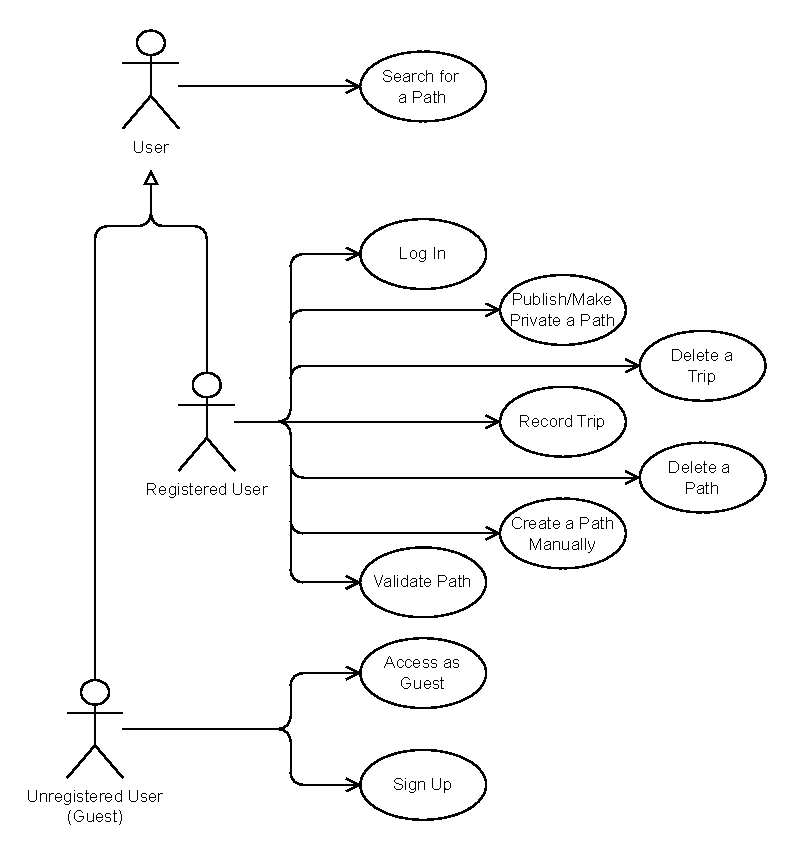
\includegraphics[width=\textwidth]{pdf/use_case_diagram.pdf}
    \caption{Use Case Diagram}
    \label{fig:use_case_diagram}
\end{figure}
\newpage
\subsection{Use Cases and Activity Diagrams}

\subsubsection*{[UC1] Sign Up by a User}
\begin{table}[H]
    \sf
    \small
    \centering
    \renewcommand{\arraystretch}{1.5}
    \begin{tabularx}{\textwidth}{|l|X|}
        \hline
        \cellcolor{lightgray} \textbf{Actor} & Unregistered User (Guest) \\
        \hline
        \cellcolor{lightgray} \textbf{Entry Conditions} & The User is not logged into the software. \\
        \hline
        \cellcolor{lightgray} \textbf{Flow of Events} & 
        \begin{enumerate}[leftmargin=*, before=\vspace*{-\baselineskip}]
            \item On the homepage, the User clicks the \emph{Sign Up} button, entering the initial registration page.
            \item The User provides the required details: name, surname and his other personal details, email, password and password confirmation.
            \item The User confirms the provided information by clicking the \emph{Register} button.
            \item The System verifies that the information is valid and that there is no existing profile associated with that email address.
            \item The System sends an OTP (One Time Password) to the email address provided to verify identity.
            \item The User enters the received OTP into the application.
            \item The System validates the OTP and activates the User's account.
            \item The User i redirected to the \emph{Explore} page.
        \end{enumerate}
        \\ 
        \hline
        \cellcolor{lightgray} \textbf{Exit Conditions} & The profile is complete and the User has access to its functionalities. \\
        \hline
        \cellcolor{lightgray} \textbf{Exceptions} & 
        \begin{itemize}[leftmargin=*, before=\vspace*{-\baselineskip}]
            \item Existing profile: If the email address provided is already associated with an account, the System will deny registration and inform the User.
            \item OTP verification failed: If the OTP entered is incorrect or does not match, the identity is not verified and the account is not activated until a correct one is provided (implicit in the verification process).
        \end{itemize}
        \\ 
        \hline
    \end{tabularx}
    \caption{UC1: Sign Up by a User}
\end{table}
\newpage
\begin{figure}[H]
    \centering
    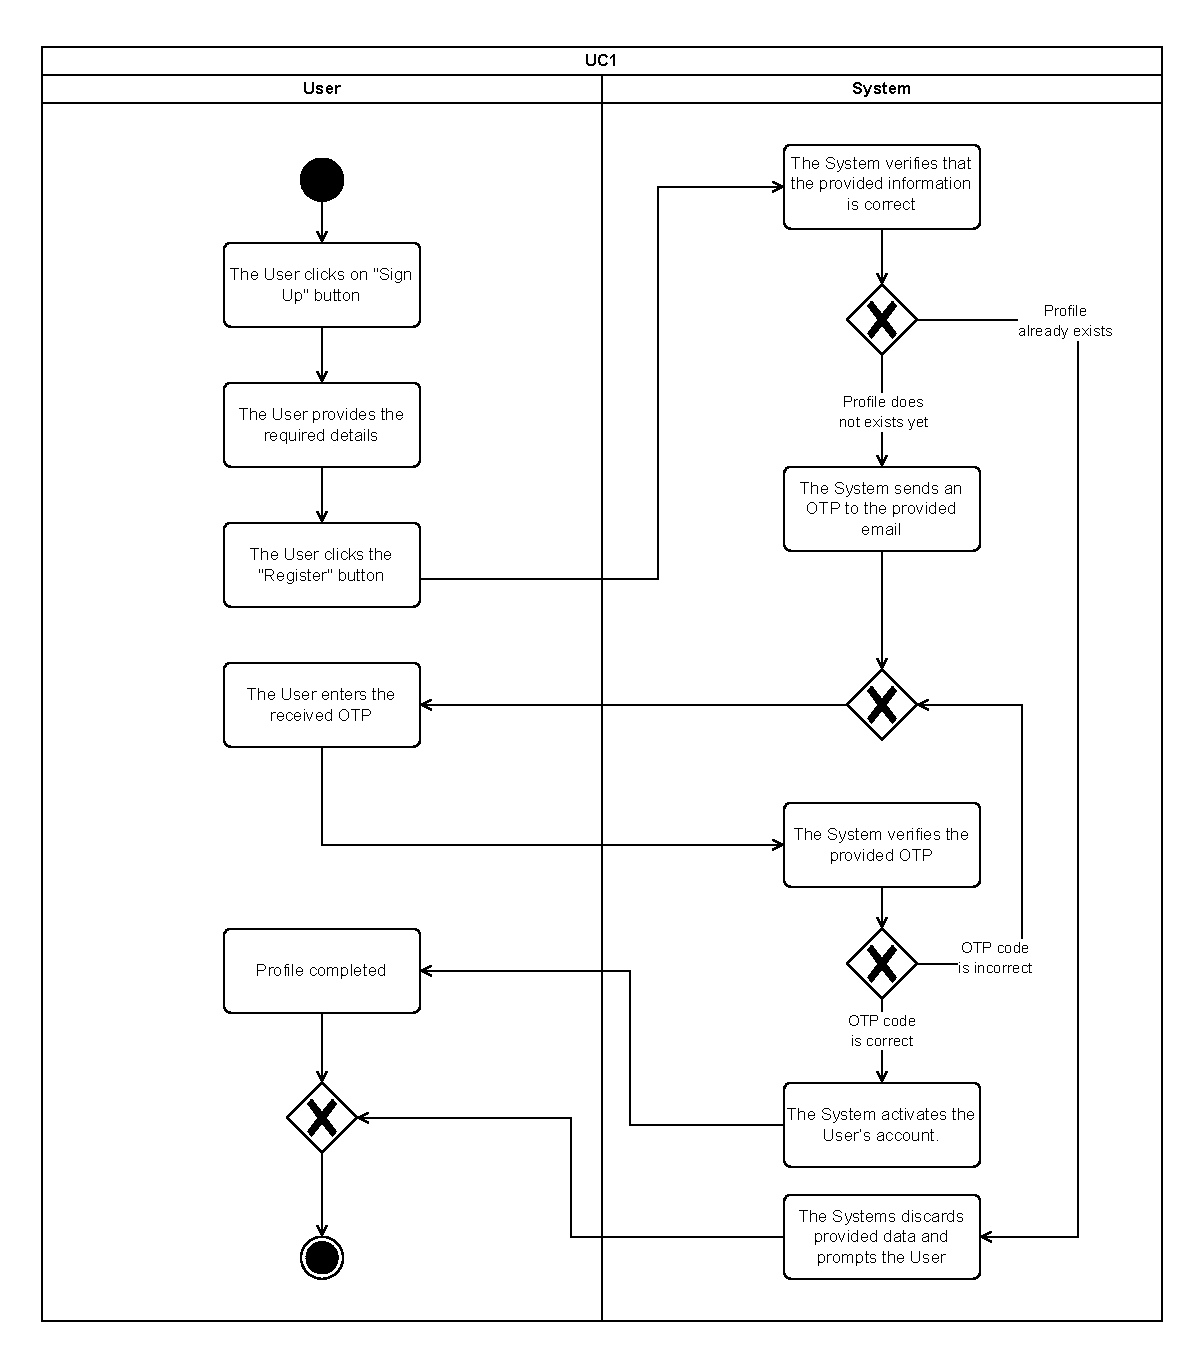
\includegraphics[width=\textwidth]{pdf/UC1.pdf}
    \caption{UC1 Activity Diagram}
    \label{fig:UC1}
\end{figure}
\newpage
\subsubsection*{[UC2] Log In by a User}
\begin{table}[H]
    \sf
    \small
    \centering
    \renewcommand{\arraystretch}{1.5}
    \begin{tabularx}{\textwidth}{|l|X|}
        \hline
        \cellcolor{lightgray} \textbf{Actor} & Registered User \\ 
        \hline
        \cellcolor{lightgray} \textbf{Entry Conditions} & The User is not already logged into the software. \\ 
        \hline
        \cellcolor{lightgray} \textbf{Flow of Events} & 
        \begin{enumerate}[leftmargin=*, before=\vspace*{-\baselineskip}]
            \item On the homepage, the User clicks the \emph{Login} button, which displays the login form.
            \item The User enters their email and password into the designated fields.
            \item The User clicks the \emph{Login} button.
            \item The System validates the provided credentials.
            \item The System redirects the User to the \emph{Explore} page.
        \end{enumerate}
        \\ 
        \hline
        \cellcolor{lightgray} \textbf{Exit Conditions} & The User is successfully logged in. \\ 
        \hline
        \cellcolor{lightgray} \textbf{Exceptions} & 
        \begin{itemize}[leftmargin=*, before=\vspace*{-\baselineskip}]
            \item Incorrect credentials: If the credentials provided are incorrect, the System denies access and prompts the User to try again.
        \end{itemize}
        \\ 
        \hline
    \end{tabularx}
    \caption{UC2: Log In by a User}
\end{table}
\newpage
\begin{figure}[H]
    \centering
    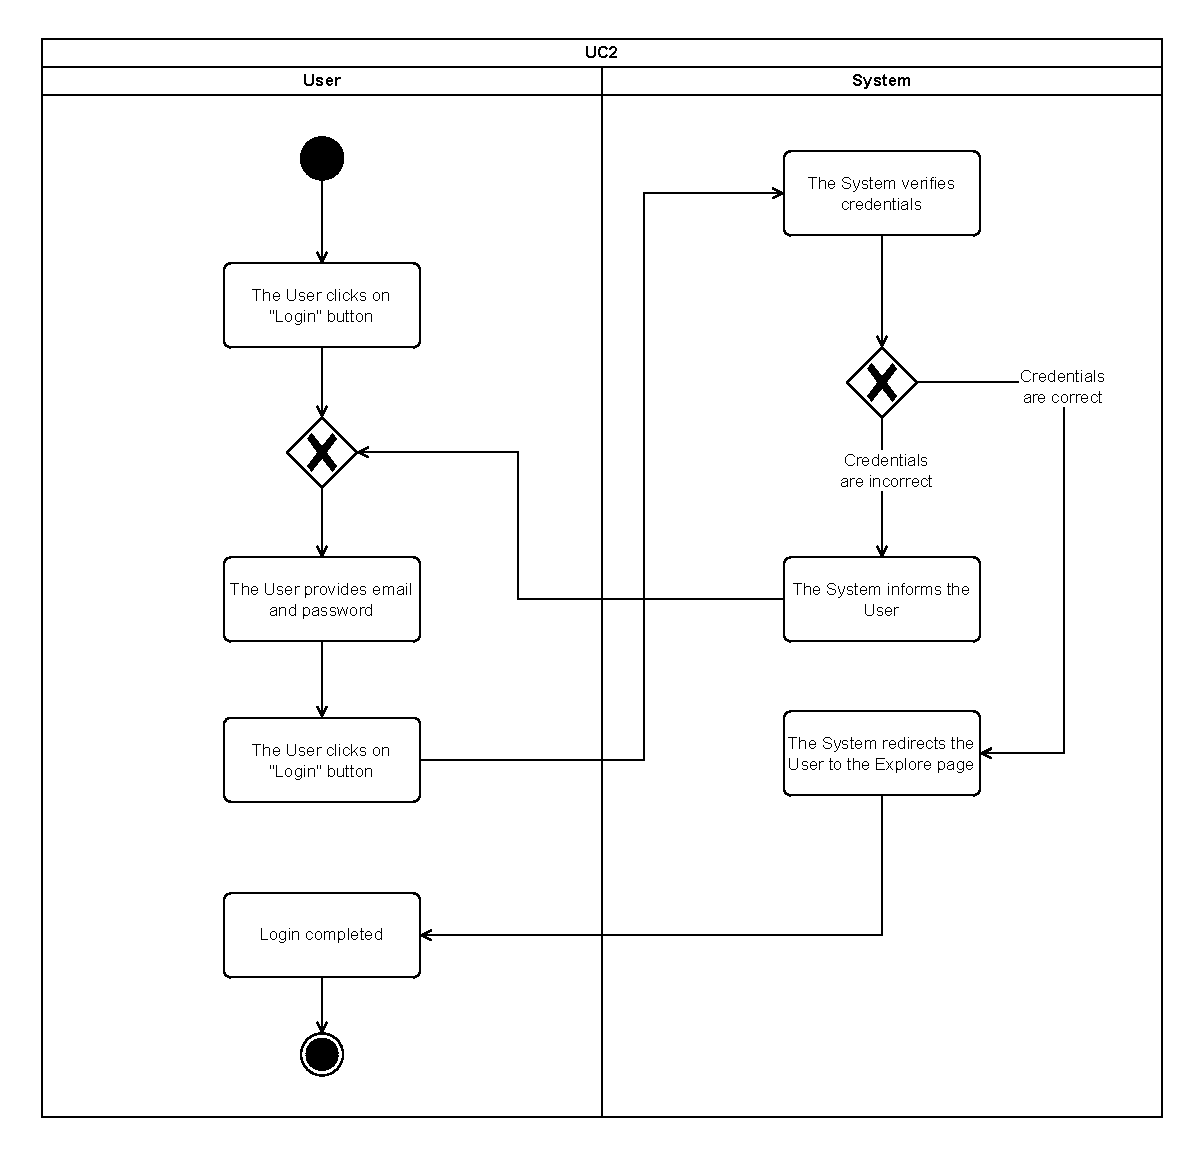
\includegraphics[width=\textwidth]{pdf/UC2.pdf}
    \caption{UC2 Activity Diagram}
    \label{fig:UC2}
\end{figure}
\newpage
\subsubsection*{[UC3] Access as Guest}
\begin{table}[H]
    \sf
    \small
    \centering
    \renewcommand{\arraystretch}{1.5}
    \begin{tabularx}{\textwidth}{|l|X|}
        \hline
        \cellcolor{lightgray} \textbf{Actor} & Unregistered User (Guest) \\ 
        \hline
        \cellcolor{lightgray} \textbf{Entry Conditions} & The User has opened the application and is on the landing screen. \\ 
        \hline
        \cellcolor{lightgray} \textbf{Flow of Events} & 
        \begin{enumerate}[leftmargin=*, before=\vspace*{-\baselineskip}]
            \item On the Login/Sign Up screen, the User selects the \emph{Continue as Guest} option.
            \item The System grants access to the public features of the application (Search, Map Visualization).
            \item The System restricts access to private features (Recording, My Activity) by hiding them or disabling the buttons.
            \item The User is redirected to the \emph{Explore} page.
        \end{enumerate}
        \\ 
        \hline
        \cellcolor{lightgray} \textbf{Exit Conditions} & The User can browse and search for Paths but cannot record data. \\ 
        \hline
    \end{tabularx}
    \caption{UC3: Access as Guest}
\end{table}
\newpage
\begin{figure}[H]
    \centering
    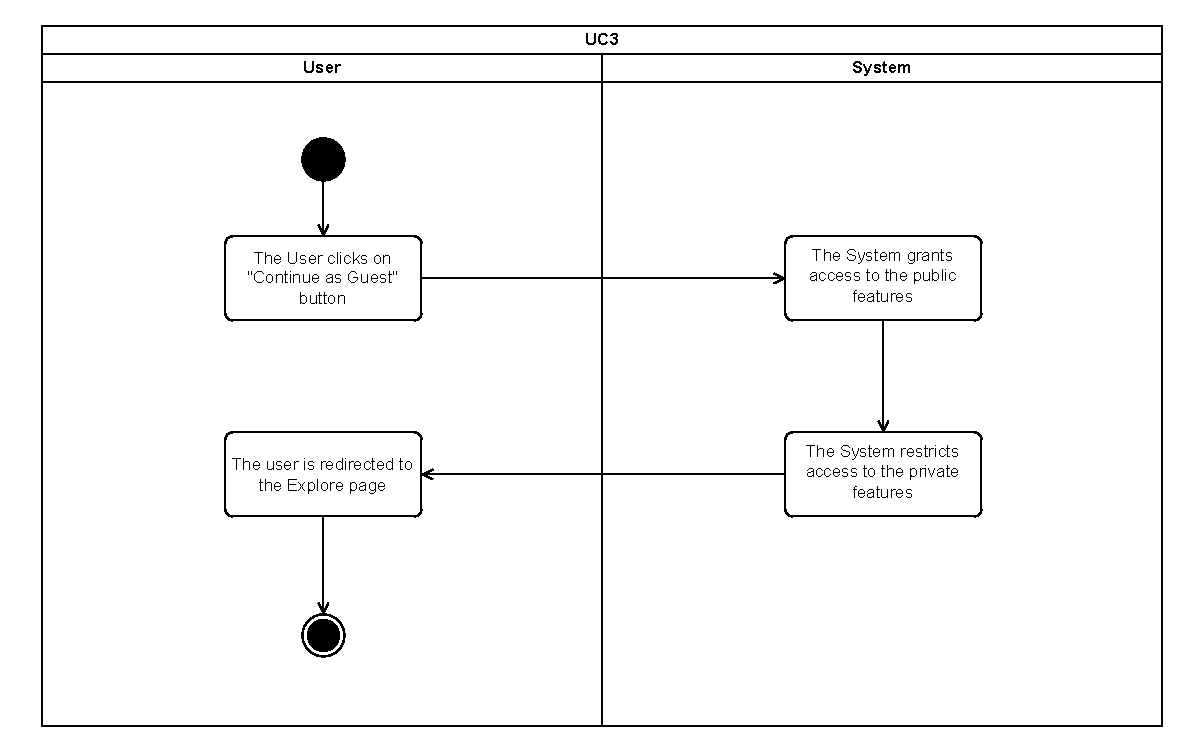
\includegraphics[width=\textwidth]{pdf/UC3.pdf}
    \caption{UC3 Activity Diagram}
    \label{fig:UC3}
\end{figure}
\newpage
\subsubsection*{[UC4] Record a Trip}
\begin{table}[H]
    \sf
    \small
    \centering
    \renewcommand{\arraystretch}{1.5}
    \begin{tabularx}{\textwidth}{|l|X|}
        \hline
        \cellcolor{lightgray} \textbf{Actor} & Registered User \\ 
        \hline
        \cellcolor{lightgray} \textbf{Entry Conditions} & The User is logged into the software. \\ 
        \hline
        \cellcolor{lightgray} \textbf{Flow of Events} & 
        \begin{enumerate}[leftmargin=*, before=\vspace*{-\baselineskip}]
            \item The User selects the \emph{Start Cycling} command to begin a session.
            \item The System automatically begins recording GPS coordinates to track the Path.
            \item While cycling, the System analyses accelerometer and gyroscope data to automatically detect potential obstacles (\eg, potholes).
            \item If the System detects that the User's speed drops below a threshold or movement indicates walking, it automatically pauses data acquisition.
            \item The System automatically resumes recording when the User starts pedalling again.
            \item The User selects the \emph{End Cycling} command to end the session.
            \item The System retrieves weather data from an external service associated with the location and time of the Trip.
            \item The System calculates performance statistics (speed, duration, distance).
            \item The System presents a Trip summary and prompts the User to validate any detected obstacles.
        \end{enumerate}
        \\ 
        \hline
        \cellcolor{lightgray} \textbf{Exit Conditions} & The Trip has been recorded, the statistics are calculated, and the Path is ready for User validation. \\ 
        \hline
        \cellcolor{lightgray} \textbf{Exceptions} & 
        \begin{itemize}[leftmargin=*, before=\vspace*{-\baselineskip}]
            \item Non-Cycling Activity: If the User never cycles (\eg, only walks), the System pauses recording and the Segment is not added to the cycling Path inventory.
        \end{itemize}
        \\ 
        \hline
    \end{tabularx}
    \caption{UC4: Record a Trip}
\end{table}
\newpage
\begin{figure}[H]
    \centering
    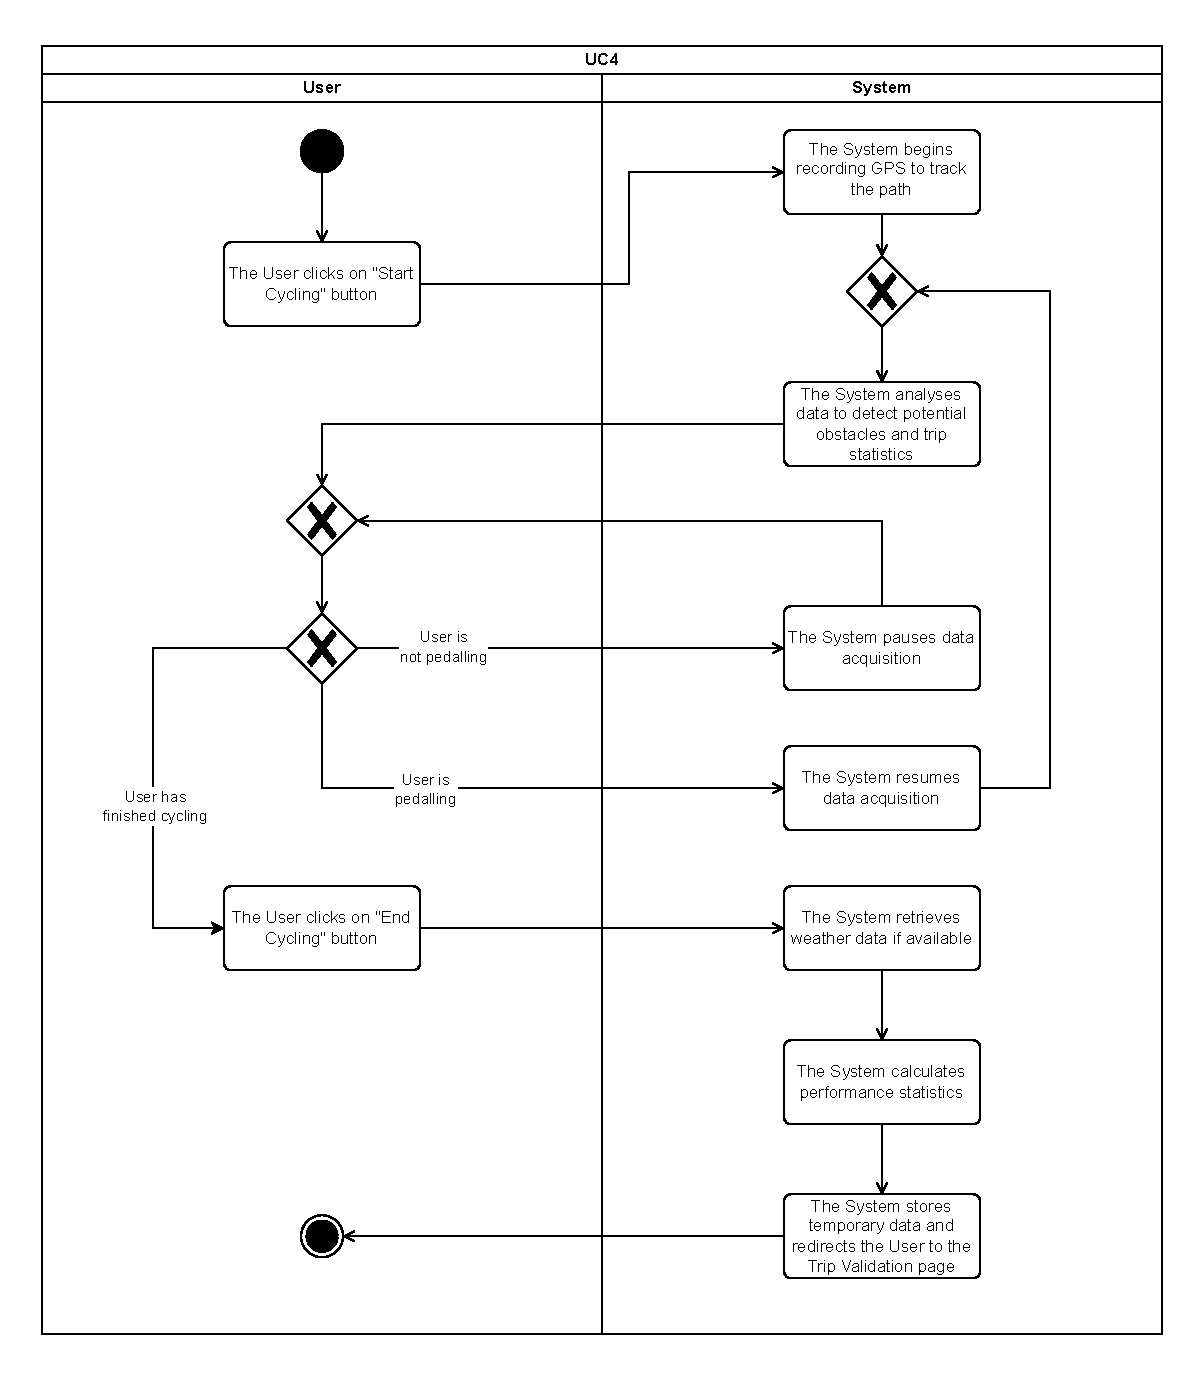
\includegraphics[width=\textwidth]{pdf/UC4.pdf}
    \caption{UC4 Activity Diagram}
    \label{fig:UC4}
\end{figure}
\newpage
\subsubsection*{[UC5] Validate a Trip and Path}
\begin{table}[H]
    \sf
    \small
    \centering
    \renewcommand{\arraystretch}{1.5}
    \begin{tabularx}{\textwidth}{|l|X|}
        \hline
        \cellcolor{lightgray} \textbf{Actor} & Registered User \\ 
        \hline
        \cellcolor{lightgray} \textbf{Entry Conditions} & The User is logged into the software and they have just finished a recording session (pressed \emph{End Cycling}). \\ 
        \hline
        \cellcolor{lightgray} \textbf{Flow of Events} & 
        \begin{enumerate}[leftmargin=*, before=\vspace*{-\baselineskip}]
            \item The System shows the User a Trip summary and any automatically detected obstacles.
            \item The User examines the proposed obstacles.
            \item The User confirms the presence of real obstacles or rejects false positives (swiping or tapping on the list).
            \item The User manually inserts any additional obstacles that the System failed to detect, pinpointing them on the map and assigning a type (\eg, \emph{Pothole}).
            \item The User assigns a general status to the Path just completed (\eg, \emph{Optimal,} \emph{Needs Maintenance}).
            \item The System applies this status to all the road Segments traversed during the Trip and,         \item Optionally, the User selects specific Segments on the map to override the general status with a more specific one (\eg, marking only one section as \emph{Needs Maintenance}).
            \item The User confirms saving the Trip and the Path and decides whether to make the Path public or private.
            \item The System permanently saves the Trip, the Path (linking the specific Segment statuses) and confirmed data in the database, preventing future changes to the GPS track. If the User opted for the publication of the Path, the System launches the aggregation algorithm: it recalculates the status of the affected road Segments by merging the User's new data with the community's existing data.
        \end{enumerate}
        \\ 
        \hline
        \cellcolor{lightgray} \textbf{Exit Conditions} & The Trip is saved and the Path is validated and saved in the User's profile; the obstacle information has been cleaned of false positives.\\ 
        \hline
        \cellcolor{lightgray} \textbf{Exceptions} & 
        \begin{itemize}[leftmargin=*, before=\vspace*{-\baselineskip}]
            \item Trip cancellation: If the User realizes that the recording is invalid, they decide to delete the entire Trip (Path included) instead of validating it. The System removes all temporary data and nothing is saved.
        \end{itemize}
        \\ 
        \hline
    \end{tabularx}
    \caption{UC5: Validate a Trip and Path}
\end{table}
\newpage
\begin{figure}[H]
    \centering
    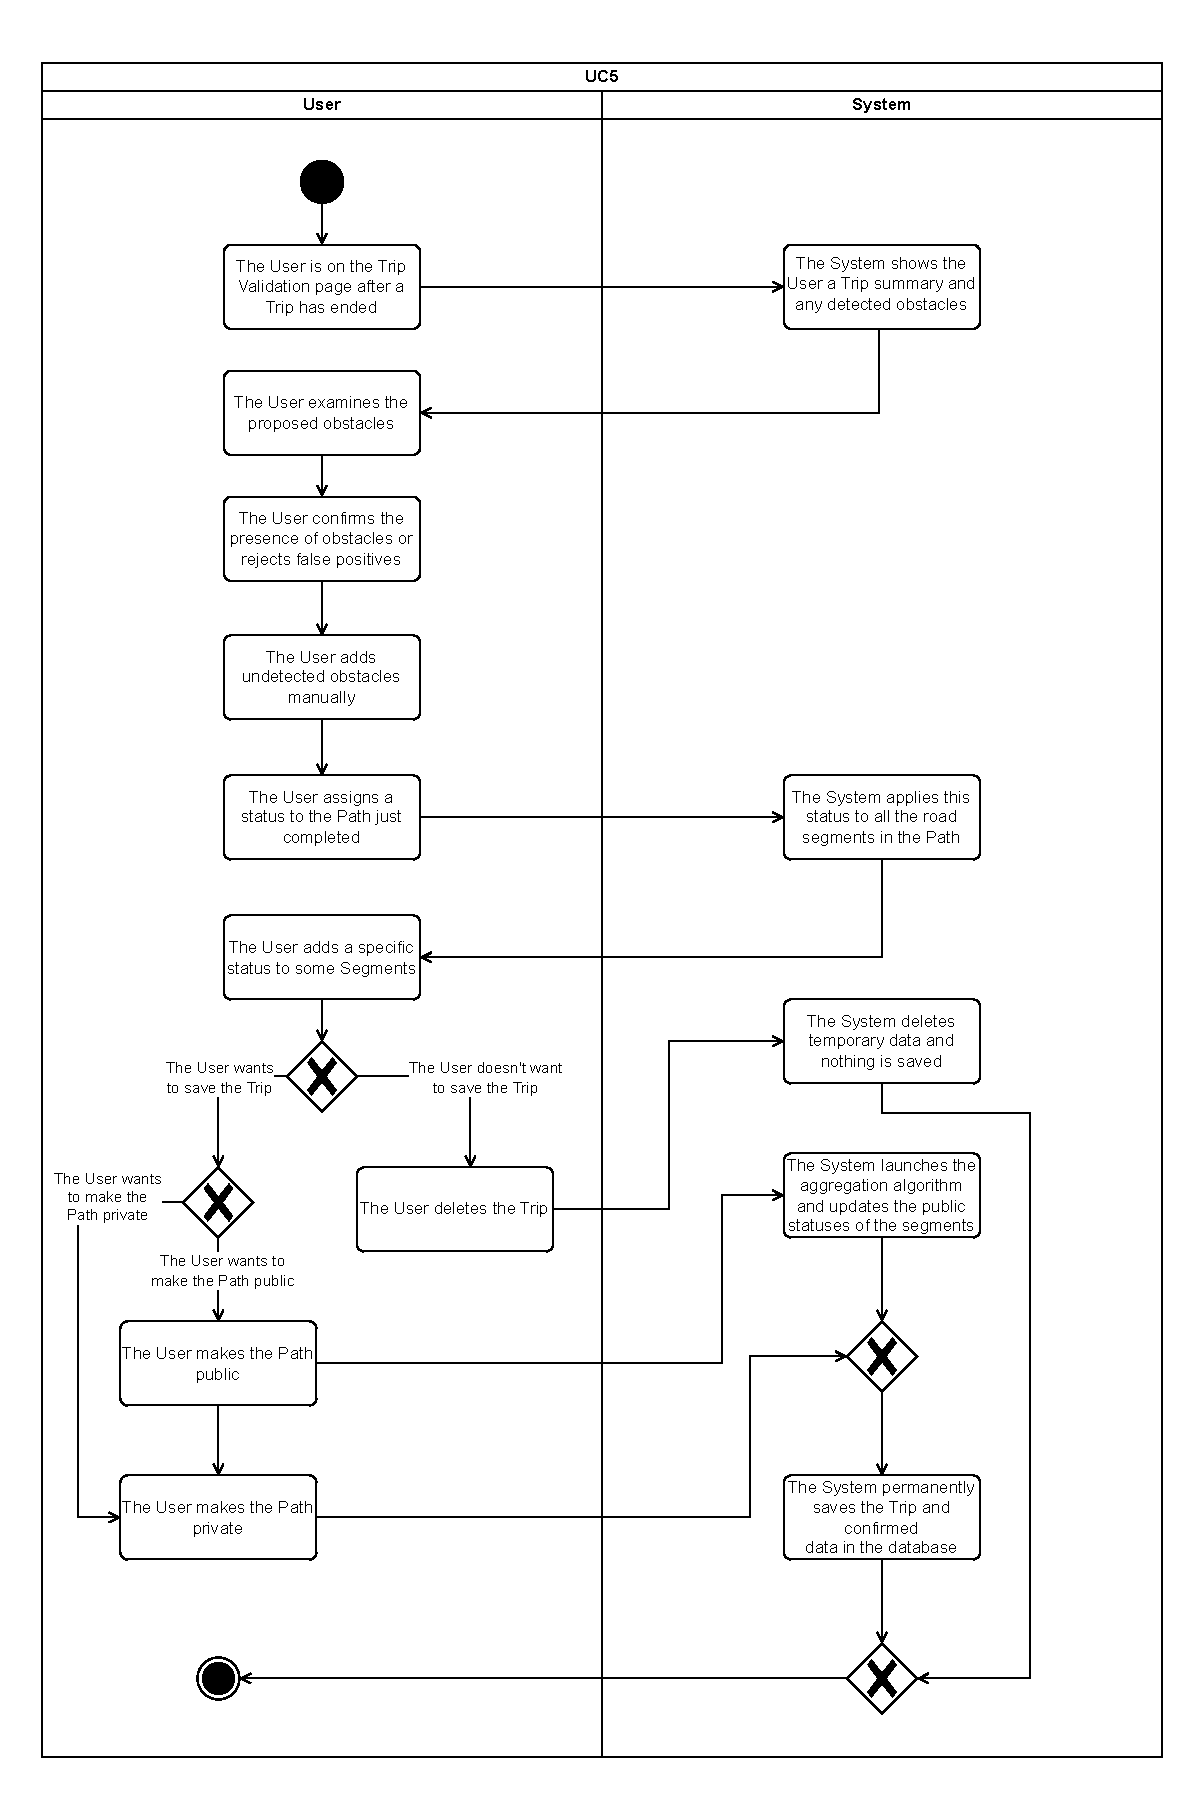
\includegraphics[width=\textwidth]{pdf/UC5.pdf}
    \caption{UC5 Activity Diagram}
    \label{fig:UC5}
\end{figure}
\newpage
\subsubsection*{[UC6] Change Path's visibility}
\begin{table}[H]
    \sf
    \small
    \centering
    \renewcommand{\arraystretch}{1.5}
    \begin{tabularx}{\textwidth}{|l|X|}
        \hline
        \cellcolor{lightgray} \textbf{Actor} & Registered User \\ 
        \hline
        \cellcolor{lightgray} \textbf{Entry Conditions} & The User has inserted a Path, either manually or automatically, and is in the Path details page. \\ 
        \hline
        \cellcolor{lightgray} \textbf{Flow of Events} & 
        \begin{enumerate}[leftmargin=*, before=\vspace*{-\baselineskip}]
            \item The User chooses the option to make the Path \emph{Public}.
            \item The System receives the request and updates the Path's visibility attribute.
            \item The System launches the aggregation algorithm: it recalculates the status of the affected road Segments by merging the User's new data with the community's existing data.
            \item The System resolves any data conflicts based on the freshness of the information and the number of confirmed reports.
            \item The System confirms to the User that the Path has been successfully published.
        \end{enumerate}
        \\ 
        \hline
        \cellcolor{lightgray} \textbf{Exit Conditions} & The Path is visible to all Users on the global map and aggregated community data (scores, road status) has been updated.\\ 
        \hline
        \cellcolor{lightgray} \textbf{Exceptions} & The Path was already public: the System will not perform any operation.\\
        \hline
    \end{tabularx}
    \caption{UC6: Change of Path's visibility}
\end{table}
Note that the described procedure outlines the process for making a Path public. However, it is also possible to revert a previously published Path to a private state in the same way. In such a case, the System would set the visibility status to \emph{private} and all related aggregated data would be restored.
\newpage
\begin{figure}[H]
    \centering
    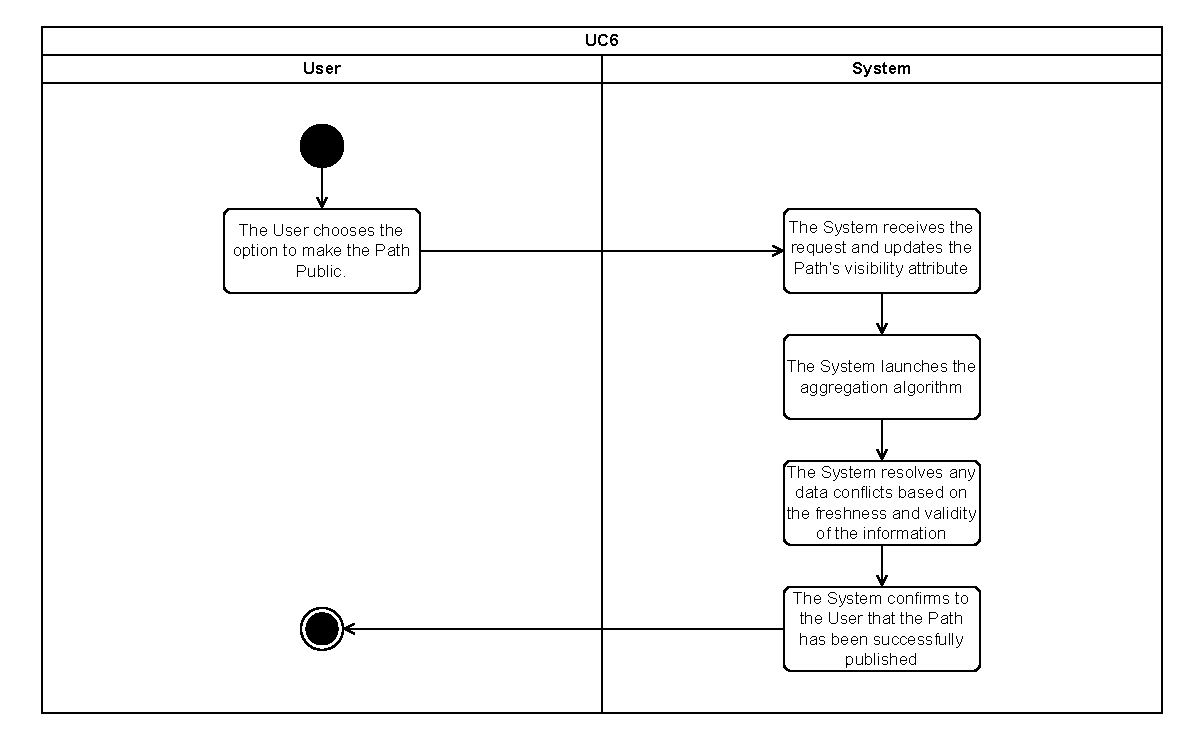
\includegraphics[width=\textwidth]{pdf/UC6.pdf}
    \caption{UC6 Activity Diagram}
    \label{fig:UC6}
\end{figure}
\newpage
\subsubsection*{[UC7] Create a Path manually}
\begin{table}[H]
    \sf
    \small
    \centering
    \renewcommand{\arraystretch}{1.5}
    \begin{tabularx}{\textwidth}{|l|X|}
        \hline
        \cellcolor{lightgray} \textbf{Actor} & Registered User \\ 
        \hline
        \cellcolor{lightgray} \textbf{Entry Conditions} & The User is logged into the software and they have selected the \emph{Create a Path} functionality.\\ 
        \hline
        \cellcolor{lightgray} \textbf{Flow of Events} & 
        \begin{enumerate}[leftmargin=*, before=\vspace*{-\baselineskip}]
            \item The User interacts with the map and manually enters the sequence of road Segments connecting an entry and exit point.
            \item The User assigns a general status to the Path (\eg, \emph{Optimal}, \emph{Hard}) to warn future cyclists.
            \item The System applies this status to all selected Segments.
            \item Optionally, the User selects specific Segments on the map to override the general status with a more specific one (\eg, marking only one section as \emph{Needs Maintenance}).
            \item The User sets the Path visibility (public/private).
            \item The User confirms Path creation.
            \item The System validates that a list of roads and statuses has been provided.
            \item The System saves the Path in the database.
            \item If set to public, the System immediately updates the global map by recalculating the aggregated status of the involved Segments.
        \end{enumerate}
        \\ 
        \hline
        \cellcolor{lightgray} \textbf{Exit Conditions} & The new Path has been saved in the System and, if public, is integrated into the global inventory of cycling Paths.\\ 
        \hline
        \cellcolor{lightgray} \textbf{Exceptions} & 
        \begin{itemize}[leftmargin=*, before=\vspace*{-\baselineskip}]
            \item Incomplete Data: If the User attempts to save without providing the road list or status, the System prevents saving and requests the missing data.
            \item Mapping Error: If the selected Segments are not contiguous or valid on the map, the System reports a tracking error.
        \end{itemize}
        \\ 
        \hline
    \end{tabularx}
    \caption{UC7: Create a Path manually}
\end{table}
\newpage
\begin{figure}[H]
    \centering
    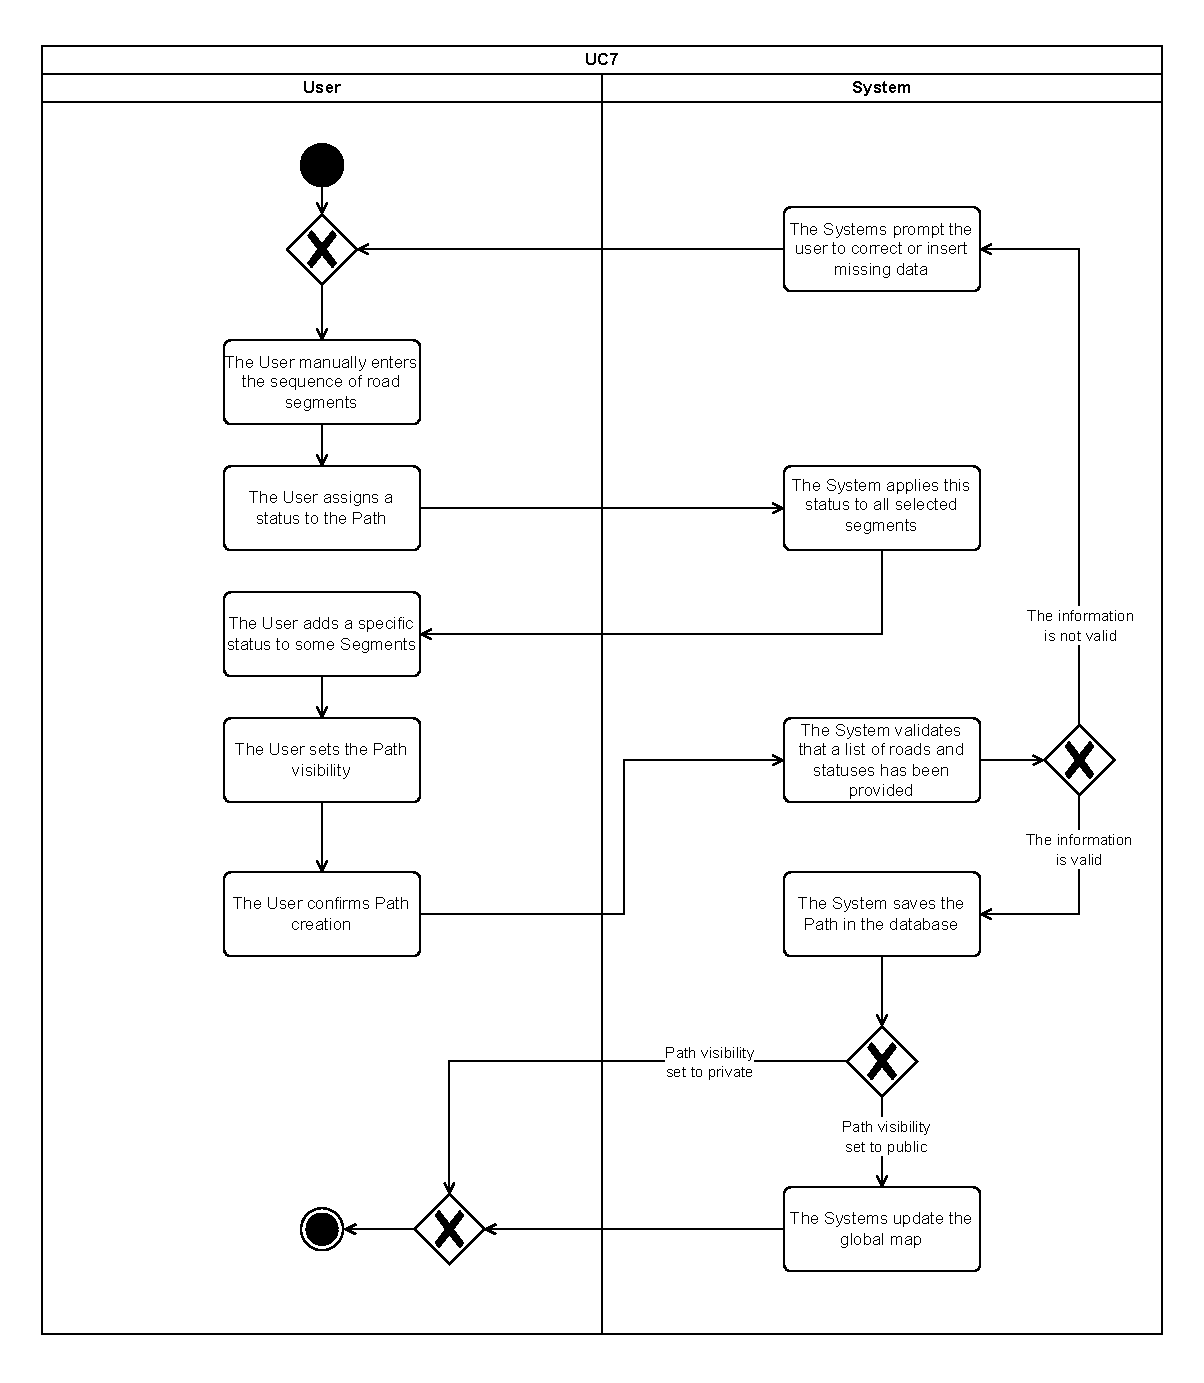
\includegraphics[width=\textwidth]{pdf/UC7.pdf}
    \caption{UC7 Activity Diagram}
    \label{fig:UC7}
\end{figure}
\newpage
\subsubsection*{[UC8] Search for a Path}
\begin{table}[H]
    \sf
    \small
    \centering
    \renewcommand{\arraystretch}{1.5}
    \begin{tabularx}{\textwidth}{|l|X|}
        \hline
        \cellcolor{lightgray} \textbf{Actor} & Guest User, Registered User \\ 
        \hline
        \cellcolor{lightgray} \textbf{Entry Conditions} & The User has access to the application and they have selected the search section. \\ 
        \hline
        \cellcolor{lightgray} \textbf{Flow of Events} & 
        \begin{enumerate}[leftmargin=*, before=\vspace*{-\baselineskip}]
            \item The User enters a source point in the search form.
            \item The User enters a destination point in the search form.
            \item The System searches the database for possible Paths connecting the two points.
            \item If multiple Paths exist, the System calculates a score for each, based on the aggregate status (\eg, presence of potholes) and the efficiency/distance to the destination.
            \item The System displays the results on a map, sorting or filtering them based on the calculated score.
            \item The User views the alternatives and selects one for details.
        \end{enumerate}
        \\ 
        \hline
        \cellcolor{lightgray} \textbf{Exit Conditions} & The User sees a list of valid Paths between the specified points, with their statuses and scores.\\ 
        \hline
        \cellcolor{lightgray} \textbf{Exceptions} & 
        \begin{itemize}[leftmargin=*, before=\vspace*{-\baselineskip}]
            \item No Path found: If there are no mapped cycling Paths between the origin and destination (or if they are not connected), the System informs the User that a Path cannot be found.
        \end{itemize}
        \\ 
        \hline
    \end{tabularx}
    \caption{UC8: Search for a Path}
\end{table}
\newpage
\begin{figure}[H]
    \centering
    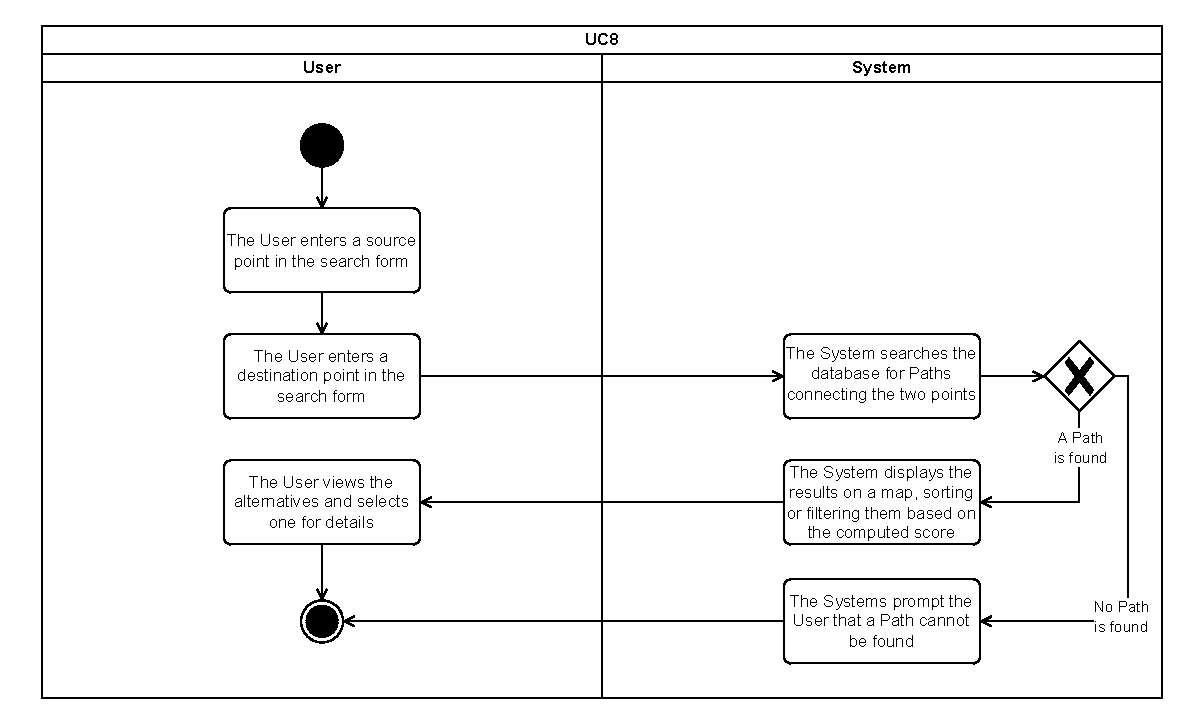
\includegraphics[width=\textwidth]{pdf/UC8.pdf}
    \caption{UC8 Activity Diagram}
    \label{fig:UC8}
\end{figure}
\newpage
\subsubsection*{[UC9] Delete a Trip}
\begin{table}[H]
    \sf
    \small
    \centering
    \renewcommand{\arraystretch}{1.5}
    \begin{tabularx}{\textwidth}{|l|X|}
        \hline
        \cellcolor{lightgray} \textbf{Actor} & Registered User \\ 
        \hline
        \cellcolor{lightgray} \textbf{Entry Conditions} & The User is logged in and has at least one recorded Trip in the \emph{My Trips} section. \\ 
        \hline
        \cellcolor{lightgray} \textbf{Flow of Events} & 
        \begin{enumerate}[leftmargin=*, before=\vspace*{-\baselineskip}]
            \item The User views the details of a specific Trip.
            \item The User presses the \emph{Delete} button.
            \item The System asks the User to choose the scope of the deletion:
                \begin{itemize}
                    \item Option A: Delete the Trip (statistics, time) but keep the Path (geometry/map).
                    \item Option B: Delete both the Trip and the associated Path.
                \end{itemize}
            \item The User selects an option and confirms the action.
            \item \textbf{Case A (Keep Path):} The System removes the Trip data (speed, duration) but retains the Path in the User's \emph{My Paths} list as a manually saved Path.
            \item \textbf{Case B (Delete Both):} The System removes both the Trip and the Path. If the Path was public, the System removes the User's contribution from the aggregated community data.
        \end{enumerate}
        \\ 
        \hline
        \cellcolor{lightgray} \textbf{Exit Conditions} & The Trip is removed. The associated Path is either preserved as an orphan entry or permanently deleted based on User choice. \\ 
        \hline
        \cellcolor{lightgray} \textbf{Exceptions} &
        \begin{itemize}[leftmargin=*, before=\vspace*{-\baselineskip}]
            \item User Cancellation: If the User cancels the confirmation prompt, no data is modified.
        \end{itemize}
        \\ 
        \hline
    \end{tabularx}
    \caption{UC9: Delete a Trip}
\end{table}
\newpage
\begin{figure}[H]
    \centering
    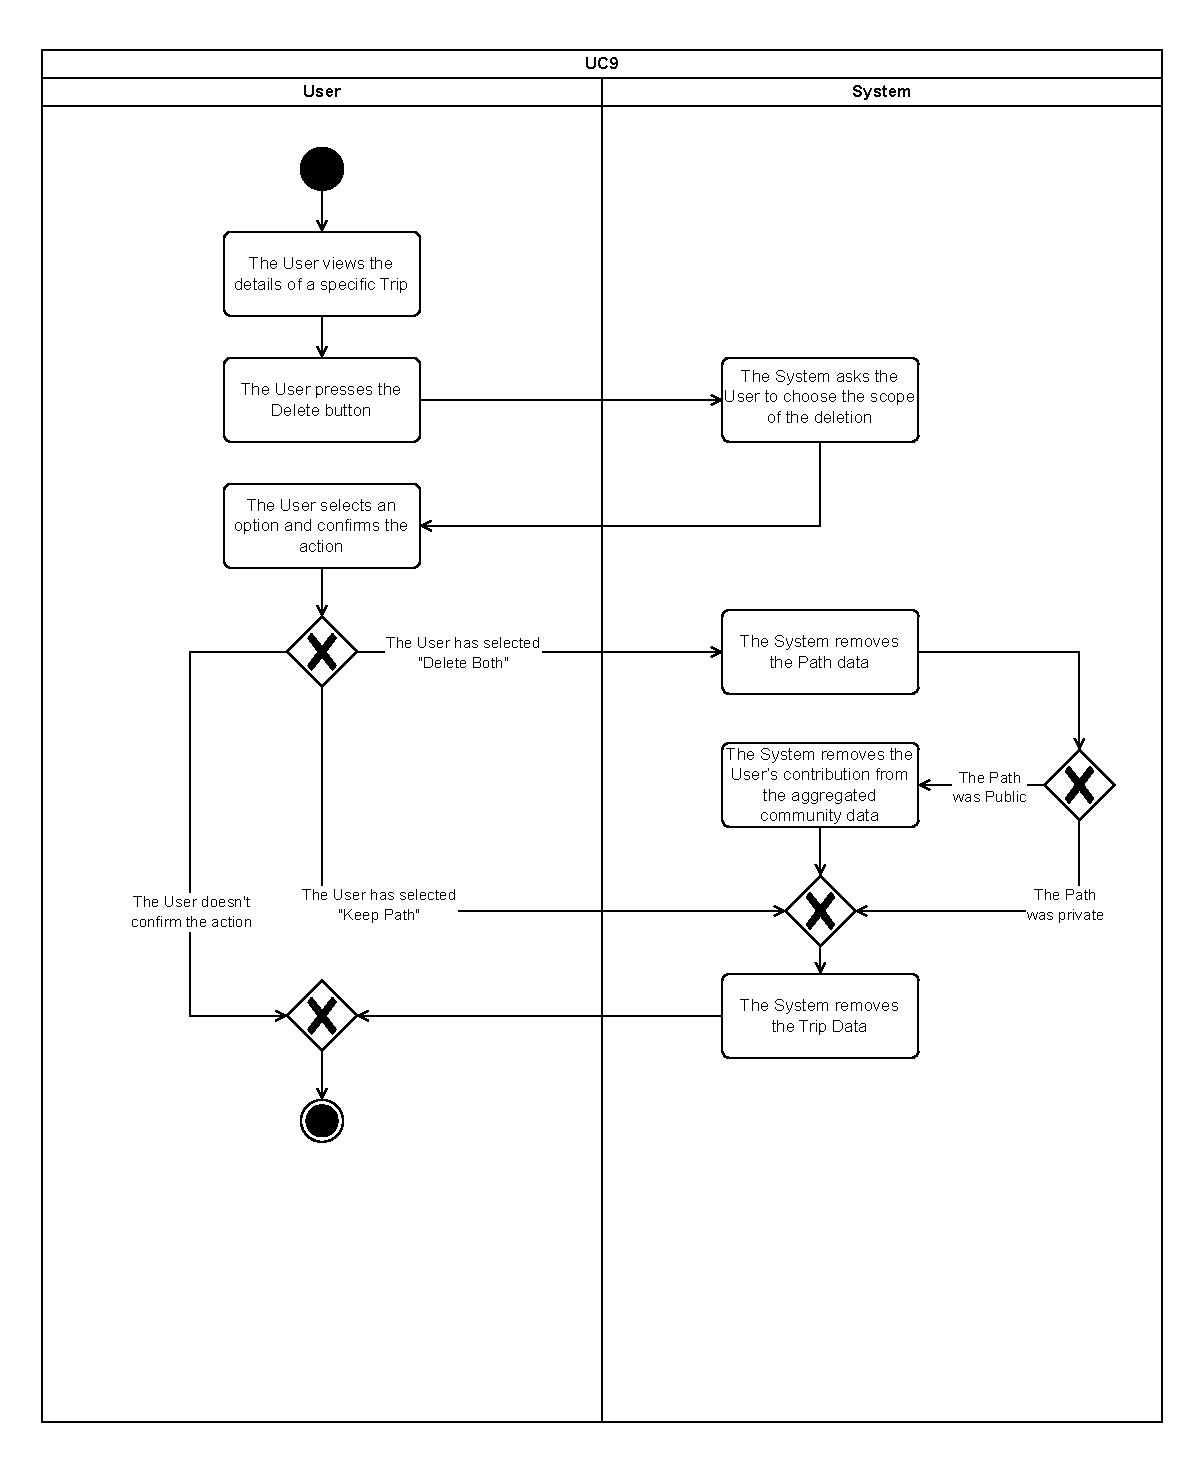
\includegraphics[width=\textwidth]{pdf/UC9.pdf}
    \caption{UC9 Activity Diagram}
    \label{fig:UC9}
\end{figure}
 \newpage
\subsubsection*{[UC10] Delete a Path}
\begin{table}[H]
    \sf
    \small
    \centering
    \renewcommand{\arraystretch}{1.5}
    \begin{tabularx}{\textwidth}{|l|X|}
        \hline
        \cellcolor{lightgray} \textbf{Actor} & Registered User \\ 
        \hline
        \cellcolor{lightgray} \textbf{Entry Conditions} & The User is logged in and has at least one Path in the \emph{My Paths} section. \\ 
        \hline
        \cellcolor{lightgray} \textbf{Flow of Events} & 
        \begin{enumerate}[leftmargin=*, before=\vspace*{-\baselineskip}]
            \item The User selects the specific Path they wish to remove.
            \item The User presses the \emph{Delete} button.
            \item The System checks for dependencies: it verifies if there is any existing recorded \emph{Trip} currently linked to this \emph{Path}.
            \item If no dependencies are found (the Path is \emph{orphan} or manually created), the System prompts for confirmation.
            \item The User confirms the operation.
            \item The System permanently removes the Path from the User's profile.
            \item If the Path was public, the System triggers the aggregate data update process to remove this contribution.
        \end{enumerate}
        \\ 
        \hline
        \cellcolor{lightgray} \textbf{Exit Conditions} & The Path is deleted from the System and removed from the global map aggregation if it was public. \\ 
        \hline
        \cellcolor{lightgray} \textbf{Exceptions} & 
        \begin{itemize}[leftmargin=*, before=\vspace*{-\baselineskip}]
            \item Dependency Error: If the System finds a \emph{Trip} associated with the Path, it blocks the deletion and displays an error message.
            \item User Cancellation: If the User denies confirmation, the Path remains intact.
        \end{itemize}
        \\ 
        \hline
    \end{tabularx}
    \caption{UC10: Delete a Path}
\end{table}
\newpage
\begin{figure}[H]
    \centering
    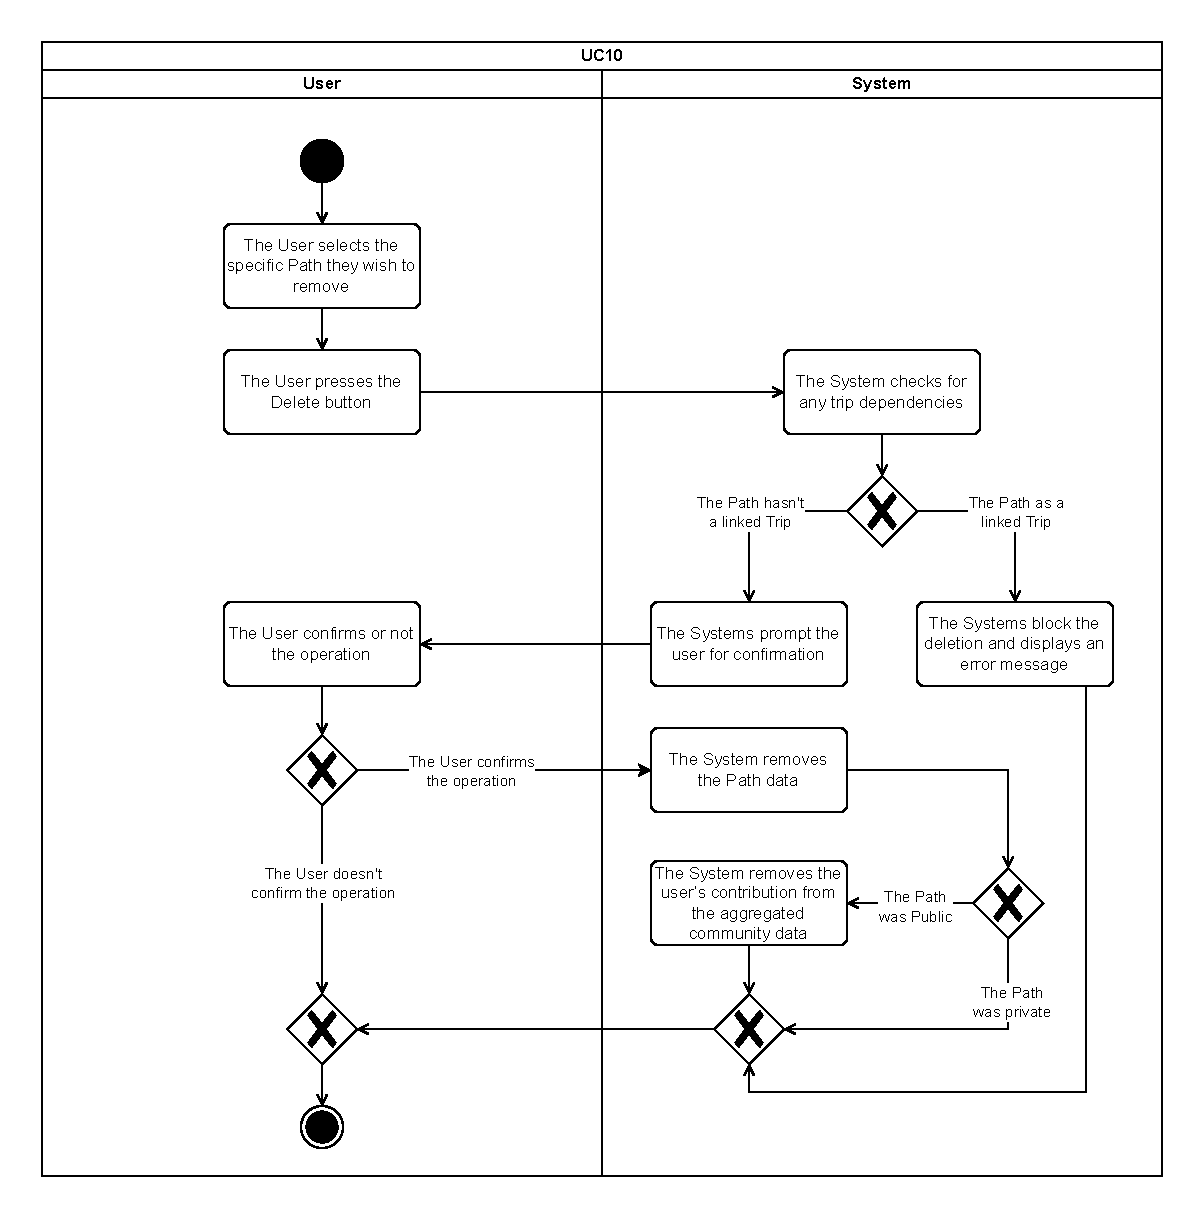
\includegraphics[width=\textwidth]{pdf/UC10.pdf}
    \caption{UC10 Activity Diagram}
    \label{fig:UC10}
\end{figure}
\newpage
\subsection{Requirement Mapping}
\begin{table}[H]
    \sf
    \small
    \centering
    \renewcommand{\arraystretch}{1.5}
    \begin{tabularx}{0.99\textwidth}{|l|X|X|X|}
        \hline
        \rowcolor{lightgray}
        \textbf{UC ID} & \textbf{Goals} & \textbf{Requirements} & \textbf{Assumptions} \\ \hline

        \textbf{UC1} & G2, G4, G8 & R1 & DA3, DA10 \\ \hline

        \textbf{UC2} & G1, G2, G3, G4, G5, G8 & R2 & DA10 \\ \hline

        \textbf{UC3} & G6, G7 & R3 & DA10 \\ \hline

        \textbf{UC4} & G1, G2, G3, G5 & R4, R5, R6, R7, R8, R9, R23, R24 & DA1, DA2, DA6, DA7, DA9, DA10 \\ \hline

        \textbf{UC5} & G2, G5, G6 & R10, R11, R12 & DA1, DA5, DA10 \\ \hline

        \textbf{UC6} & G6, G8 & R16, R17, R19, R20, R21 & DA4, DA5, DA10 \\ \hline

        \textbf{UC7} & G4, G8 & R13, R19 & DA4, DA5, DA8, DA10 \\ \hline

        \textbf{UC8} & G6, G7 & R25, R26 & DA2, DA8, DA10 \\ \hline

        \textbf{UC9} & G2, G6 & R14, R18, R22 & DA10 \\ \hline

        \textbf{UC10} & G4, G6 & R15, R18, R22 & DA10 \\ \hline    
    \end{tabularx}
    \caption{Requirements Mapping}
    \label{tab:requirements_mapping}
\end{table}
\section{Performance Requirements}
Given the mixed nature of the System (real-time sensing on the client, heavy data aggregation on the server), the performance requirements are defined as follows:

\begin{itemize}
    \item \textbf{Response Time for Interactive Tasks}: 
    For standard User interactions (\eg, Log In, accessing \emph{My Trips}, viewing a static map), the System shall respond to the User request within \textbf{1 second} under normal load conditions (excluding network latency).

    \item \textbf{Path Search Latency}: 
    Due to the computational complexity of the routing algorithm (which factors in scores, status, and distance), the System shall provide a list of suggested Paths between two locations within \textbf{5 seconds} for 95\% of requests.

    \item \textbf{Sensor Processing Latency (Client-side)}: 
    To ensure the spatial accuracy of detected obstacles, the mobile application shall process accelerometer and gyroscope variations and associate them with the current GPS coordinate with a latency not exceeding \textbf{200 milliseconds}.

    \item \textbf{Data Aggregation Freshness}: 
    The \emph{Merging Algorithm} responsible for updating Path statuses based on new User reports shall run continuously or in short bursts. The System shall ensure that a validated report from a User is reflected in the global public statistics (and thus visible to other Users) within \textbf{10 minutes} of the data upload.

    \item \textbf{System Capacity and Scalability}: 
    The backend infrastructure shall support at least \textbf{10,000 concurrent Users} (recording Trips or searching for Paths) without degradation of the response times specified above. The architecture must be horizontally scalable to handle seasonal peaks (\eg, spring/summer weekends).

    \item \textbf{Synchronization Latency}: 
    Upon restoration of internet connectivity following a period of offline activity, the application shall automatically synchronize locally cached data with the central server. The upload of a typical 1-hour Trip log (including GPS sequence, sensor metadata, and timestamps) must complete in less than \textbf{30 seconds} over a standard 4G/LTE connection.
\end{itemize}

\section{Design Requirements}
\subsection{Standards compliance}
\label{standards-compliance}
The System is designed to adhere to the following standards and regulations to ensure legal compliance, User privacy, and store eligibility:

\begin{enumerate}
    \item \textbf{General Data Protection Regulation (GDPR)}:
    As the Platform processes sensitive geolocation and sensor data, strict adherence to GDPR is enforced. Key measures include:
    \begin{itemize}
        \item \textbf{Data Anonymization}: Removing personal identifiers from Trip data before aggregation.
        \item \textbf{Data Minimization}: Collecting only the data strictly necessary for the service provision.
        \item \textbf{User Rights}: Mechanisms for Users to access, rectify, and delete their data (Right to be Forgotten).
        \item \textbf{Consent}: Explicit and granular consent collection processes for background tracking.
        \item \textbf{Transparency}: Clear data usage policies accessible within the app.
    \end{itemize}

    \item \textbf{Apple App Store Review Guidelines}:
    The iOS application must comply with Apple's strict standards to ensure approval. Focus areas include:
    \begin{itemize}
        \item \textbf{Safety (User Generated Content)}: Implementation of filtering or reporting mechanisms for offensive or malicious Path descriptions created by Users.
        \item \textbf{Privacy (Location Services)}: Compliance with guidelines for requesting background location access only when necessary and with a clear visual indicator.
        \item \textbf{Performance}: Ensuring the app does not excessively drain the battery or generate excessive heat during tracking.
    \end{itemize}

    \item \textbf{Google Play Developer Policy}:
    The Android application must adhere to Google's policies, specifically:
    \begin{itemize}
        \item \textbf{Permissions Policy}: Justifying the use of sensitive permissions as core functionality.
        \item \textbf{User Data}: Secure handling of personal information and prominent disclosure of data access.
        \item \textbf{Monetization and Ads}: Compliance with policies regarding any future promotional content, ensuring it does not interfere with app usability.
    \end{itemize}

    \item \textbf{Web Content Accessibility Guidelines (WCAG) 2.1}:
    To ensure inclusivity for Users with disabilities, the mobile interface design follows the W3C principles where applicable to mobile contexts:
    \begin{itemize}
        \item \textbf{Perceivable}: Providing text alternatives for non-text content (\eg, map icons) and sufficient colour contrast ratios (Level AA).
        \item \textbf{Operable}: Ensuring all functionalities are accessible via assistive technologies (\eg, VoiceOver, TalkBack).
        \item \textbf{Understandable}: Using clear navigation labels and readable fonts that support dynamic resizing.
    \end{itemize}
\end{enumerate}

\subsection{Hardware limitations}
The design and implementation of the BBP mobile application must account for the physical and technical constraints inherent to mobile devices:

\begin{itemize}
    \item \textbf{Battery Consumption}: 
    Continuous access to the GPS module and high-frequency sampling of the accelerometer and gyroscope are highly energy-intensive operations. To prevent rapid battery drainage during long cycling sessions, the application must implement optimization strategies. These include:
    \begin{itemize}
        \item Adaptive sampling rates (\eg, reducing sensor polling frequency when the User is stationary or paused).
        \item Efficient background processing to minimize CPU wake-locks.
    \end{itemize}
    
    \item \textbf{Sensor Accuracy and Heterogeneity}: 
    The quality, sensitivity, and calibration of hardware sensors (accelerometer, gyroscope) vary significantly across different device models and manufacturers. The obstacle detection algorithm must be robust enough to handle signal noise and varying hardware specifications without generating excessive false positives. Furthermore, GPS accuracy may degrade in specific environments (\eg, dense forests, urban canyons), requiring software-side compensation (\eg, map matching) to ensure Path coherence.
    
    \item \textbf{Local Storage Capacity}: 
    To support the caching of the Path while cycling, the application relies on the device's internal storage. The System must implement efficient data compression and cache management policies to avoid exceeding reasonable storage quotas on User devices with limited capacity.
    
    \item \textbf{Thermal Constraints}: 
    Intensive processing of sensor data combined with screen usage under direct sunlight (typical for cycling) can lead to device overheating. The application logic must be optimized to minimize computational load, preventing the operating System from throttling performance or shutting down the app for thermal protection.
\end{itemize}
\subsection{Any other constraint}
\begin{itemize}
    \item \textbf{Network Connectivity and Volatility}: 
    As established in the \hyperref[domain_assumptions]{Domain Assumptions}, the application is frequently used in environments with unstable or absent cellular coverage (\eg, rural areas, mountain trails). Therefore, the System architecture involves a constraint on data synchronization: non-critical operations (\eg, uploading Trip data, downloading map updates) must be deferrable and capable of resuming automatically when connectivity is restored (\emph{Store and Forward} mechanism).

    \item \textbf{Third-Party API Rate Limits}: 
    The System relies on external services for map tiles and weather data. To maintain operational sustainability and avoid service denial due to exceeding quota limits (Rate Limiting), the System must implement strict caching policies (\eg, caching weather data for a specific area for 1 hour instead of refreshing it at every request).

    \item \textbf{Safety and Liability Disclaimer}: 
    Since the application suggests physical Paths and relies on User generated content which might be outdated or subjective, the System interface is constrained to display a mandatory safety disclaimer upon startup. The System must explicitly inform Users that Path suggestions are for informational purposes only and do not replace adherence to local traffic laws or personal judgment of road conditions.
\end{itemize}
\section{Software System Attributes}

\subsection{Reliability}
To guarantee dependable performance, the System must capably manage errors and rapidly recover from interruptions, thereby reducing overall downtime, the frequency of issues, and the impact on specific features. This requirement shall be fulfilled by utilizing \textbf{industry-standard fault-tolerance protocols} (specifically through the \textbf{redundancy} of data storage and processing nodes) to \textbf{eliminate single points of failure}.

\subsection{Availability}
The backend System must maintain a \textbf{minimum uptime of 99\%} (2-nines), limiting unscheduled outages to a maximum of 3.65 days annually. The server-side service must remain accessible at all times, with the exception of planned maintenance windows scheduled during off-peak hours and communicated in advance. 
However, regarding the client-side mobile application, the System shall allow Users to record Trips and acquire sensor data even in the \textbf{absence of internet connectivity}, \textbf{locally caching} the information and \textbf{synchronizing} it with the central server once the connection is restored. This ensures the primary function (tracking) is available even in remote areas. 

\subsection{Security}
The System is required to implement \textbf{secure authentication} using email and password credentials, alongside \textbf{authorization mechanisms} to verify identities and restrict feature access according to User roles. These controls shall be enforced through rigorous password policies and encrypted communication protocols such as \textbf{HTTPS}. Furthermore, the Platform must guarantee \textbf{data integrity} by prohibiting unauthorized modifications to preserve the accuracy of information. To ensure \textbf{confidentiality}, sensitive data must be \textbf{encrypted both in transit and at rest}, rendering it unreadable in the event of interception or exposure. Additionally, the System must remain resilient against standard attack vectors, including \textbf{SQL injection, XSS, and CSRF}, while incorporating regular security patches to mitigate new vulnerabilities.

\subsection{Maintainability}
A maintenance schedule must be established to accommodate hardware/software upgrades, new feature deployment, bug resolution, and security patching. These operations are expected to average 8 hours in duration, targeting \textbf{off-peak traffic windows}, and must strictly adhere to a \textbf{24-hour maximum limit}. Major maintenance events are to be considered exceptions, occurring no more than two to three times annually, and require a public announcement at least 48 hours prior. Furthermore, software maintainability shall be ingrained in the development lifecycle from the outset through the enforcement of industry best practices. The resulting codebase must be \textbf{clean, modular, reusable, and loosely coupled} to streamline the future integration of new functionalities.

\subsection{Portability}
The System is designed as a \textbf{Cross-Platform Mobile Application}, ensuring compatibility with the two major mobile operating Systems (\textbf{Android and iOS}) through a \textbf{unified codebase} (\eg, using frameworks like Flutter or React Native). This approach guarantees a consistent User experience across different devices while minimizing development and maintenance efforts compared to maintaining two separate native codebases. 
Furthermore, the choice of a mobile app architecture over a web-based one is dictated by the requirement to access \textbf{native hardware features}, specifically the accelerometer, gyroscope, and GPS background services, with high performance and reliability, which are essential for the automated obstacle detection features.

\chapter{Formal Analysis Using Alloy}
\label{chap:alloy_analysis}

\section{The Model Structure}
The formal Model has been developed using \textbf{Alloy 6}, leveraging its support for Linear Temporal Logic (LTL) to verify the dynamic behaviour of the System. The code is organized into modular files to enhance readability and maintainability: signatures, predicates, facts, assertions, and a main execution module.
The primary goal of this Model is to verify the correctness of the algorithm responsible for updating Segment status upon the publication of a Path, ensuring data consistency and isolation between Users.

\subsection{Signatures}
This module defines the structural atoms and the state of the System. A \emph{var} keyword is used to model mutable elements that evolve over time steps.
The representation abstracts away certain details to focus on the core verification goals:
\begin{itemize}
    \item \textbf{Users:} Only registered Users are modelled, as Guest Users operate in a read-only mode that does not alter the System state.
    \item \textbf{Obstacles:} These are omitted as they are static attributes in this context and do not influence the dynamic propagation of visibility and status logic.
    \item \textbf{PathEntries:} These are abstracted away. In the \hyperref[section:domain_class_diagram]{domain model}, a Path is composed of entries; in this formal Model, the Path's status is applied directly to the set of involved Segments. This abstraction simplifies the state space without compromising the logic of the propagation algorithm.
\end{itemize}

\begin{code}
    \inputminted{alloy}{code/signatures.als}
\end{code}

\subsection{Predicates}
This module outlines the possible state transitions (operations) within the System. A representative subset of actions has been selected to model the critical lifecycle of Paths and Trips.
Operations such as account deletion or unpublishing a Path are excluded from this abstraction. This design choice allows the Model to focus specifically on the \emph{safety} and \emph{liveness} properties of the publication workflow without the complexity of edge cases that do not affect the core update algorithm.
Each predicate defines strict pre-conditions and post-conditions to guide the solver.

\begin{code}
    \inputminted{alloy}{code/predicates.als}
\end{code}

\subsection{Facts}
This file contains the Model invariants and consistency conditions. These rules enforce:
\begin{itemize}
    \item \textbf{Structural Integrity:} Constraints that must hold true in every state (\eg, a Path must contain at least one Segment).
    \item \textbf{System Trace:} The definition of allowed temporal evolutions using LTL.
    \item \textbf{Consistency Conditions:} Rules ensuring that variables not explicitly modified by an operation remain unchanged (\emph{inertia}), preventing unwanted side effects.
\end{itemize}

\begin{code}
    \inputminted{alloy}{code/facts.als}
\end{code}

\subsection{Assertions}
This module encodes the properties that must be verified against the Model.
Rather than representing the full complexity of the real-world implementation, these assertions are tailored to the abstracted Model to formally prove:
\begin{itemize}
    \item \textbf{Safety:} Bad things never happen (\eg, a User cannot publish another User's Path).
    \item \textbf{Liveness:} Good things eventually happen (\eg, Segment status is updated correctly).
    \item \textbf{Possibility:} Valid states are reachable (\eg, Segment sharing between Paths is possible).
\end{itemize}

\begin{code}
    \inputminted{alloy}{code/assertions.als}
\end{code}

\subsection{Main Execution}
This file serves as the entry point for the Alloy Analyser. It contains the \texttt{run} commands to generate specific trace scenarios and the \texttt{check} commands to validate the assertions against the logic defined in the previous modules.

\begin{code}
    \inputminted{alloy}{code/main.als}
\end{code}

\newpage
\section{Validation through the Model}
This section illustrates the validation results obtained from the Alloy Analyzer. Instances generated by the \texttt{run} commands demonstrate the consistency of the Model, while the assertion checks verify the safety and liveness properties of the System.


\subsection{Large Static World}
The execution of the \texttt{run largeStaticWorld} command successfully produced a consistent instance, confirming that the structural axioms allow for a populated System state without contradictions.
Figure \ref{fig:large_static_model} depicts a meaningful snapshot of the System generated by the Analyser, featuring multiple Users, Paths, and Segments satisfying the multiplicity constraints.
\begin{figure}[H]
    \centering
    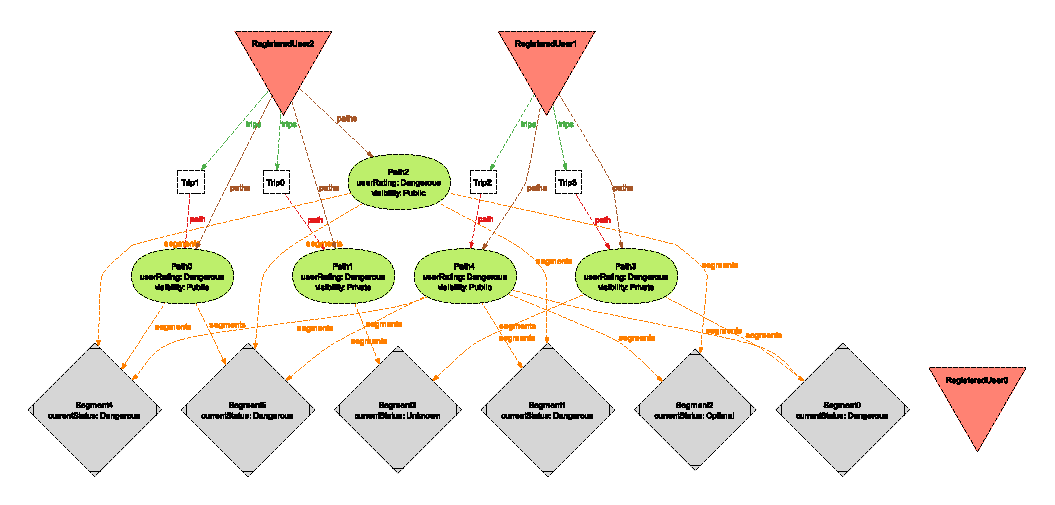
\includegraphics[width=\textwidth]{RASDv1.0/pdf/large_static_world.pdf}
    \caption{Large Static World Instance}
    \label{fig:large_static_model}
\end{figure}


\subsection{Dynamic World}
The \texttt{run dynamicWorld} command generates a trace satisfying the Linear Temporal Logic (LTL) specifications defined in the \emph{SystemTrace} fact. The following figures illustrate the step-by-step evolution of the System state.

\begin{figure}[H]
    \centering
    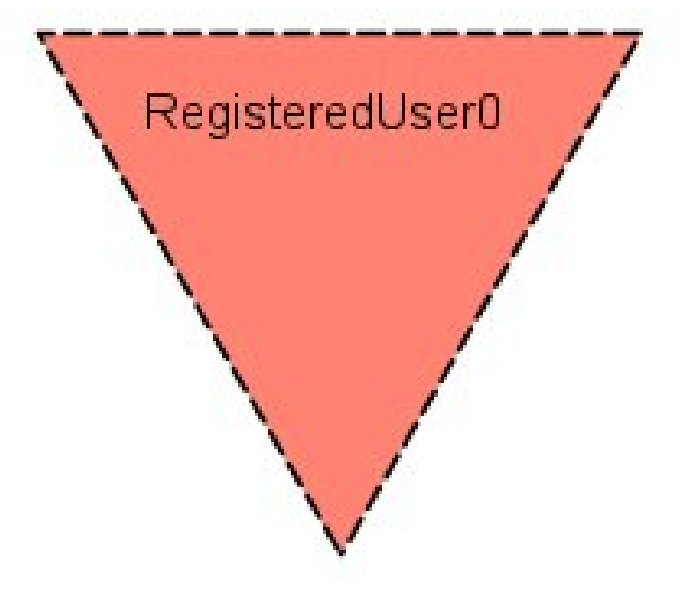
\includegraphics[width=0.2\textwidth]{RASDv1.0/pdf/dynamic_world_1.pdf}
    \caption{Dynamic World, Step 1: System Initialization and Sign Up}
    \label{fig:dynamic_1}
\end{figure}
\noindent
The trace begins in Figure \ref{fig:dynamic_1} with the initialization of the universe and the \texttt{signUp} of the first User.

\begin{figure}[H]
    \centering
    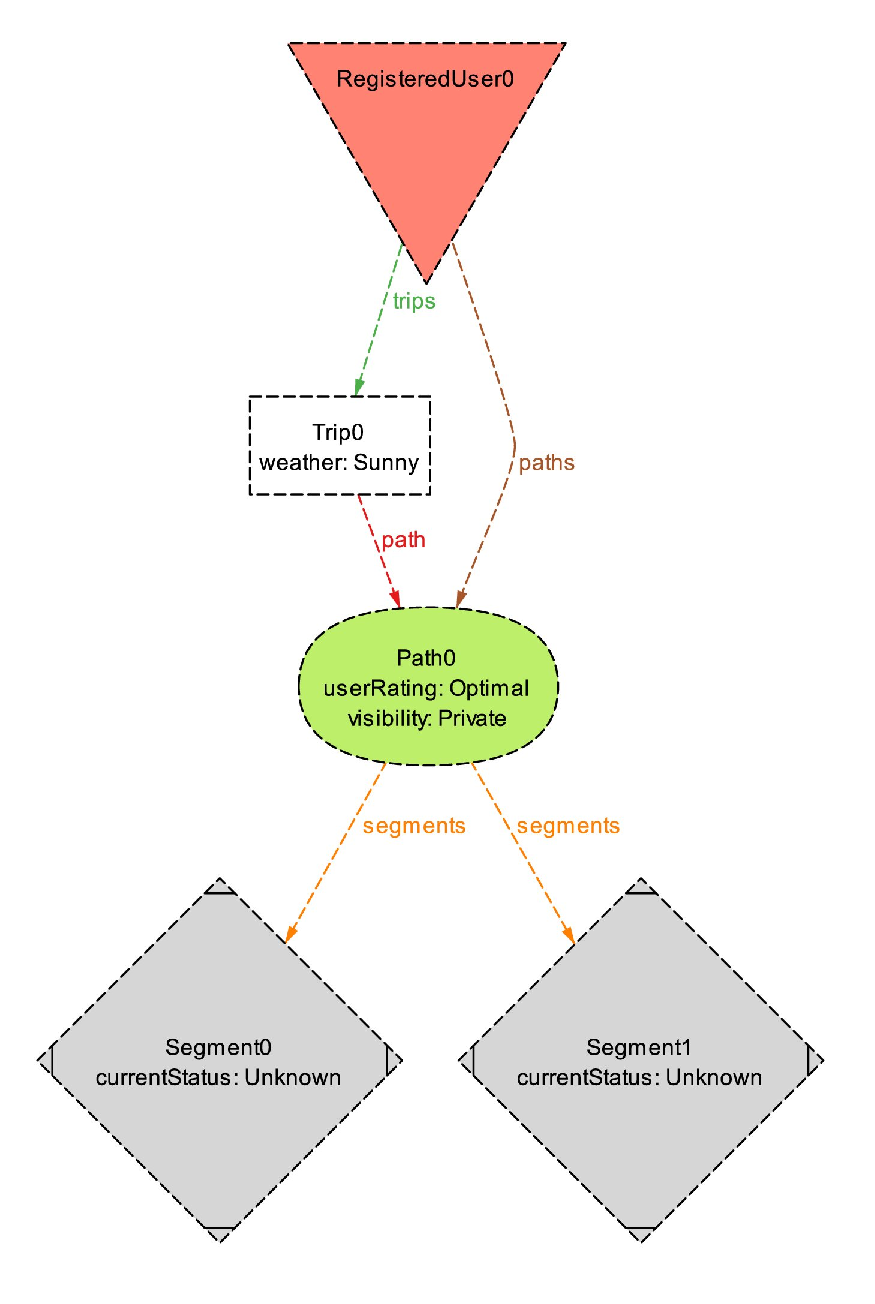
\includegraphics[width=0.4\textwidth]{RASDv1.0/pdf/dynamic_world_2.pdf}
    \caption{Dynamic World, Step 2: Trip Recording}
    \label{fig:dynamic_2}
\end{figure}
\noindent
In Figure \ref{fig:dynamic_2}, User 0 records a Trip. This action triggers the creation of a new Path and the instantiation of the corresponding Segments.

\begin{figure}[H]
    \centering
    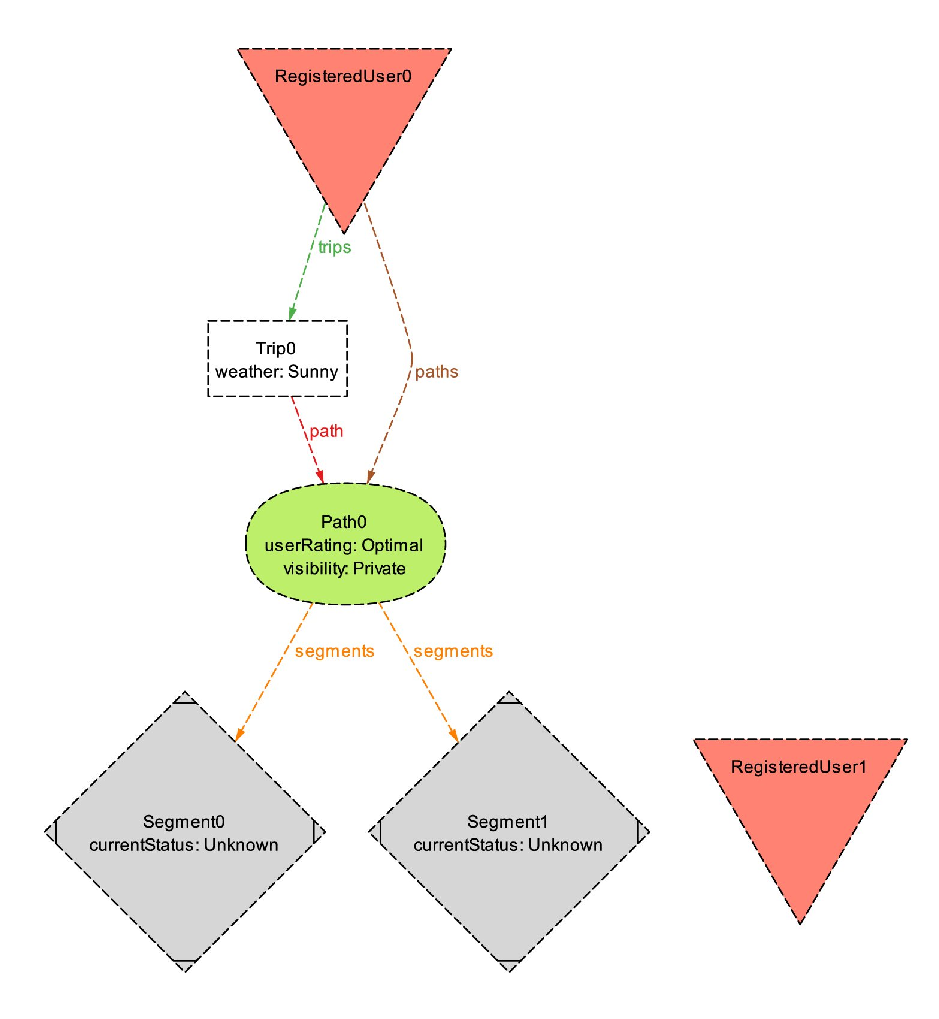
\includegraphics[width=0.5\textwidth]{RASDv1.0/pdf/dynamic_world_3.pdf}
    \caption{Dynamic World, Step 3: User 1 Sign Up}
    \label{fig:dynamic_3}
\end{figure}
\noindent
Figure \ref{fig:dynamic_3} shows the expansion of the User base with the registration of User 1.

\begin{figure}[H]
    \centering
    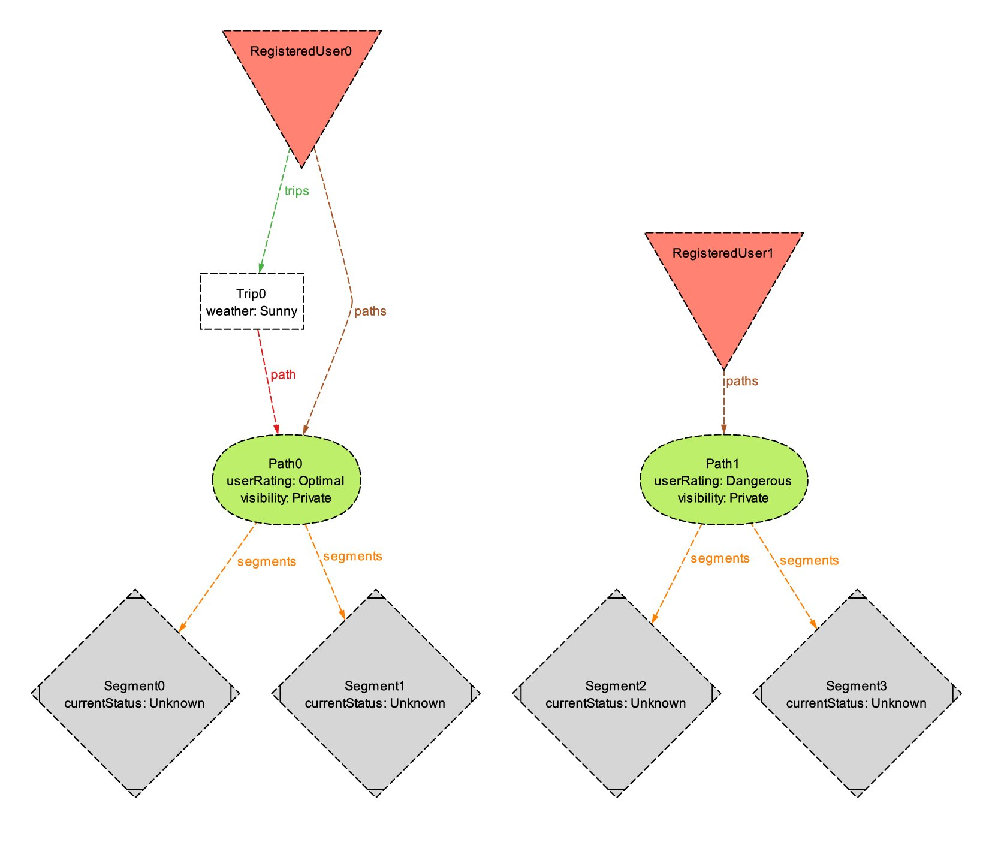
\includegraphics[width=0.7\textwidth]{RASDv1.0/pdf/dynamic_world_4.pdf}
    \caption{Dynamic World, Step 4: Manual Path Creation}
    \label{fig:dynamic_4}
\end{figure}
\noindent
In Figure \ref{fig:dynamic_4}, User 1 creates a manual Path. At this stage, the Path is private and its Segments are initialized with an \emph{Unknown} status.

\begin{figure}[H]
    \centering
    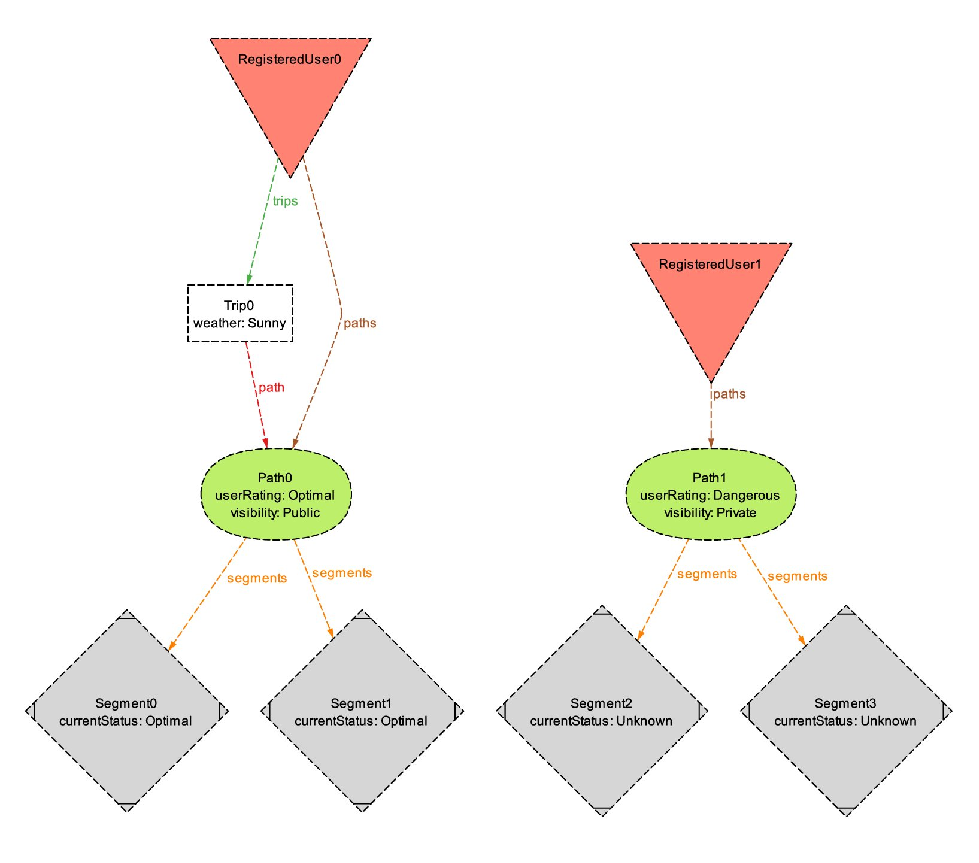
\includegraphics[width=0.7\textwidth]{RASDv1.0/pdf/dynamic_world_5.pdf}
    \caption{Dynamic World, Step 5: Path Publication}
    \label{fig:dynamic_5}
\end{figure}
\noindent
Figure \ref{fig:dynamic_5} illustrates the publication of User 0's Path. It is crucial to observe the side effect on the involved Segments: their status is updated from \emph{Unknown} to the rating provided by the User, propagating the information to the System.

\begin{figure}[H]
    \centering
    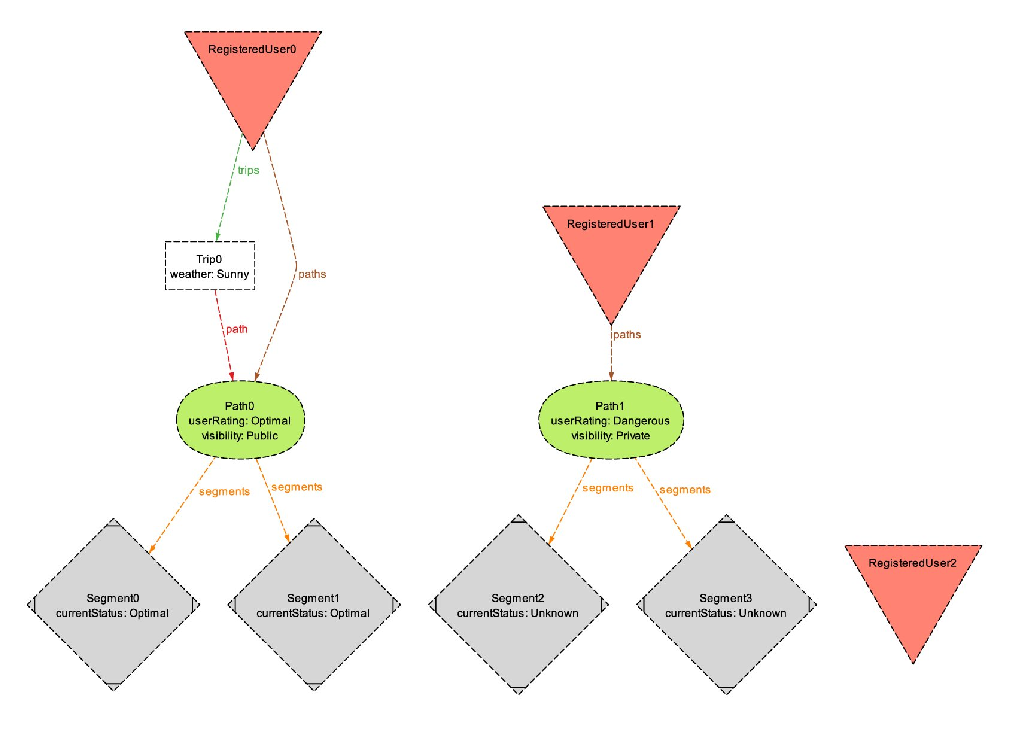
\includegraphics[width=0.85\textwidth]{RASDv1.0/pdf/dynamic_world_6.pdf}
    \caption{Dynamic World, Step 6: User 3 Sign Up}
    \label{fig:dynamic_6}
\end{figure}
\noindent
The scenario continues in Figure \ref{fig:dynamic_6} with the registration of a third User (User 3).

\begin{figure}[H]
    \centering
    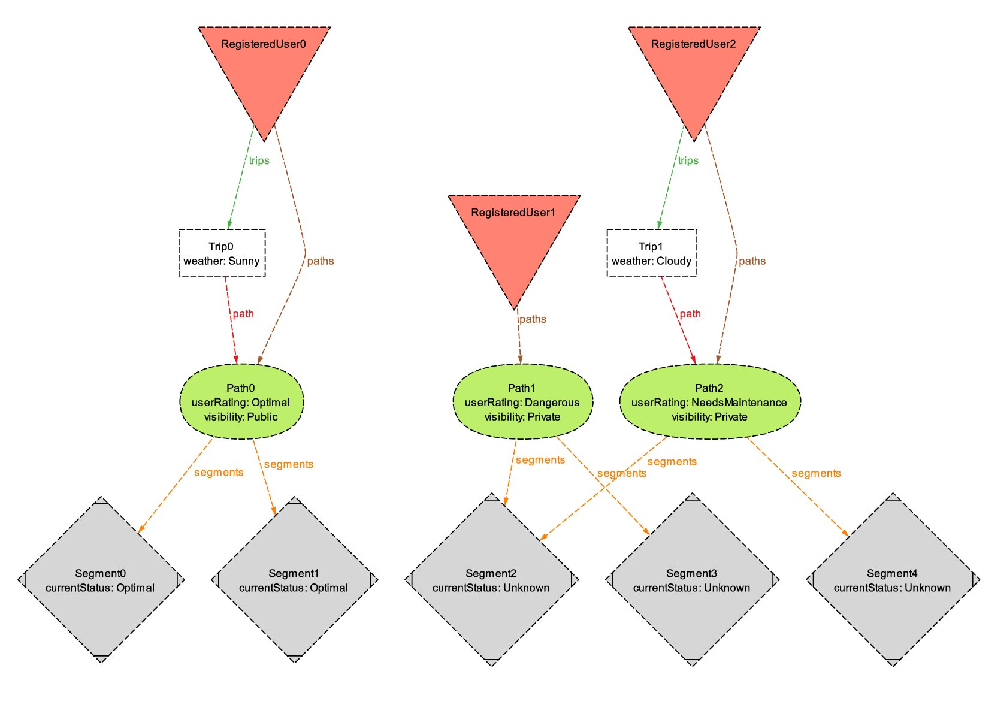
\includegraphics[width=0.85\textwidth]{RASDv1.0/pdf/dynamic_world_7.pdf}
    \caption{Dynamic World, Step 7: User 3 records a Trip}
    \label{fig:dynamic_7}
\end{figure}
\noindent
Figure \ref{fig:dynamic_7} highlights the Segment reuse logic. User 3 records a Trip that utilizes Segments already present in the System. Note that the private recording does not alter the status of these shared Segments, preserving the integrity of public data.

\begin{figure}[H]
    \centering
    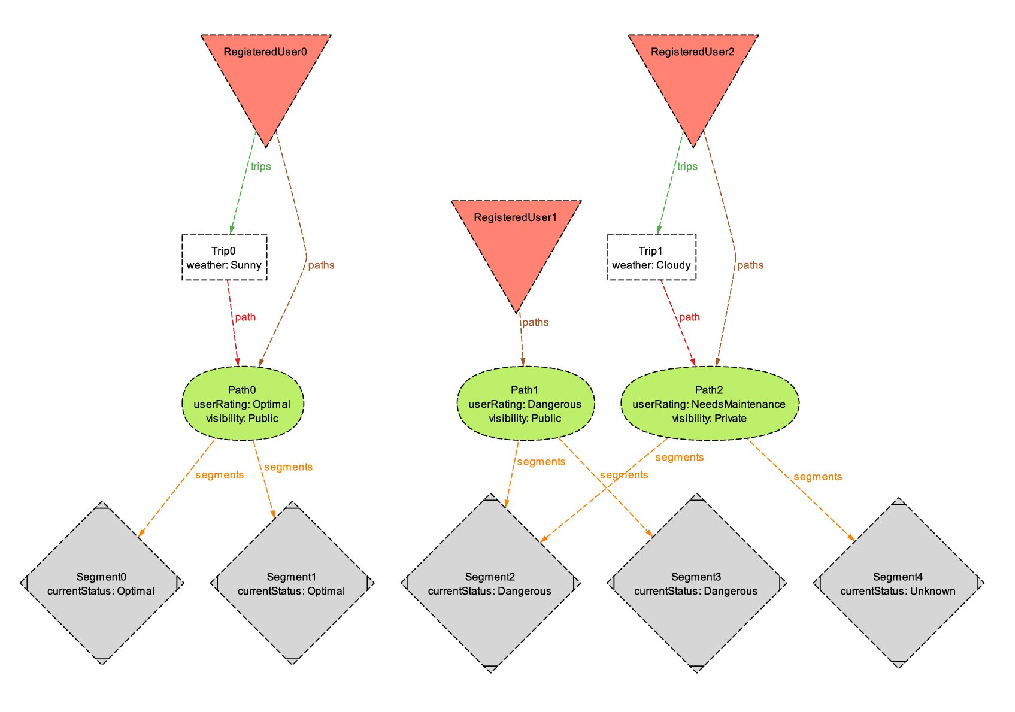
\includegraphics[width=0.9\textwidth]{RASDv1.0/pdf/dynamic_world_8.pdf}
    \caption{Dynamic World, Step 8: Second Publication}
    \label{fig:dynamic_8}
\end{figure}
\noindent
Figure \ref{fig:dynamic_8} shows the publication of User 1's Path, which updates the status of its specific Segments.

\begin{figure}[H]
    \centering
    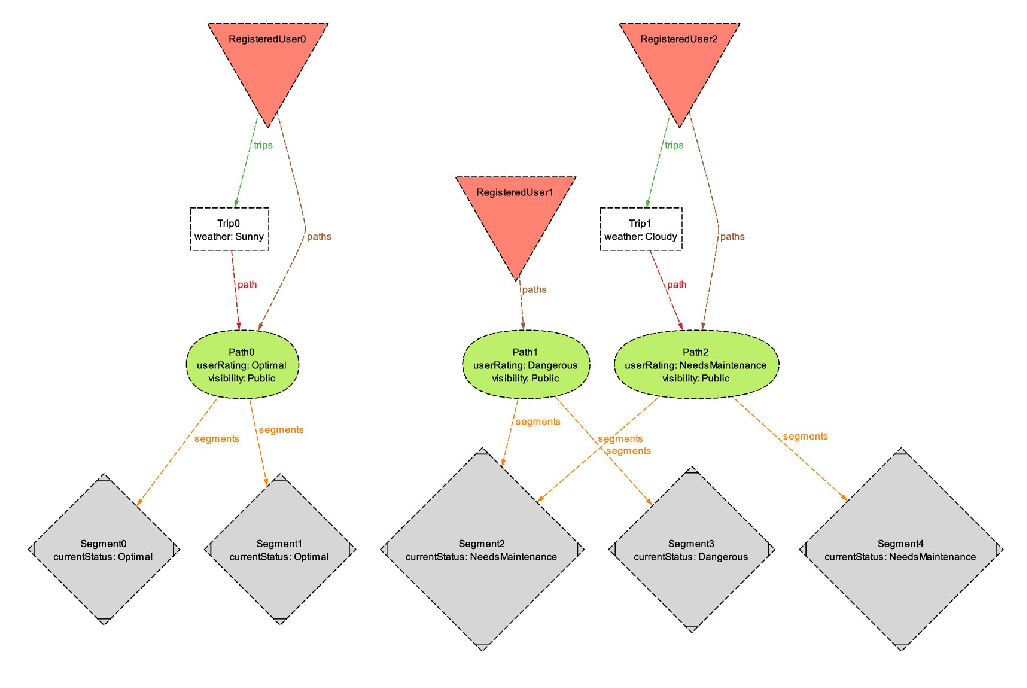
\includegraphics[width=0.9\textwidth]{RASDv1.0/pdf/dynamic_world_9.pdf}
    \caption{Dynamic World, Step 9: Third Publication}
    \label{fig:dynamic_9}
\end{figure}
\noindent
Finally, Figure \ref{fig:dynamic_9} shows the publication of User 2's Path, which updates the status of its specific Segments, overriding previous statuses, demonstrating that multiple publications can coexist without interference.

\subsection{Assertion Checks}
The formal properties of the Model were verified using the \texttt{check} command. The analyzer produced the following output:

\begin{code}
    \begin{minted}[frame=single]{alloy}
No counterexample found. VisibilityIsolation may be valid.
No counterexample found. SegmentsStatusSync may be valid.
No counterexample found. OncePublicAlwaysPublic may be valid.
Counterexample found. SharingIsImpossible is invalid.
    \end{minted}
\end{code}
\noindent
The results are fully consistent with the design requirements:
\begin{itemize}
    \item The absence of counterexamples for the first three assertions confirms the \textbf{Safety}, \textbf{Liveness}, and \textbf{Possibility} properties (isolation of User data, correct status synchronization, and monotonicity of public visibility).
    \item The counterexample found for \texttt{SharingIsImpossible} is a desired result and serves as a \textbf{constructive proof}. By refuting the impossibility of sharing, the Model demonstrates that states where Paths share Segments are reachable and valid, confirming the correct implementation of the reuse logic.
\end{itemize}

\chapter{Effort Spent}
\begin{table}[H]
    \sf
    \small
    \centering
    \renewcommand{\arraystretch}{1.5}
    \begin{tabularx}{\textwidth}{|X|X|X|X|X|}
        \hline
        \rowcolor{lightgray} \textbf{Author} & \textbf{Section 1} & \textbf{Section 2} & \textbf{Section 3} & \textbf{Section 4} \\
        \hline
        \textbf{Daniele Toniolo} & 5 & 7 & 19 & 1 \\
        \textbf{Stefano Ungaro} & 5 & 8 & 22 & 19 \\
        \textbf{Matteo Zappa} & 5 & 7.5 & 22 & 1 \\
        \hline
    \end{tabularx}
    \caption{Effort spent by each team member (unit is hours)}
\end{table}

\chapter{References}
\section{Used Tools}
\begin{itemize}
    \item \textbf{Overleaf}\footnote{\url{https://www.overleaf.com}}: \LaTeX \xspace text editor for collaborative writing.
    \item \textbf{draw.io}\footnote{\url{https://www.draw.io}}: creation of UML diagrams.
    \item \textbf{Alloy Analyser 6.2.0}\footnote{\url{https://www.alloytools.org}}: formal analysis and model checking of the system.
    \item \textbf{Google Gemini 3 Pro}\footnote{\url{https://gemini.google.com}}: used for grammar, style, and coherence checks. Prompts included specific sections of this document with instructions to analyse and refine the text based on academic standards and logical consistency.
\end{itemize}

\end{document}